\documentclass[10pt,a4paper]{article}
\usepackage[T1]{fontenc}
\usepackage[utf8]{inputenc}
\usepackage{lmodern}
\usepackage[margin=2.1cm]{geometry}
\usepackage{microtype}
\usepackage{amsmath,amssymb}
\usepackage{booktabs,longtable,array,tabularx}
\usepackage{enumitem}
\usepackage{xcolor}
\usepackage{needspace}
\usepackage{tikz}
\usetikzlibrary{arrows.meta,positioning,calc,fit}
\usepackage{caption}
\usepackage{parskip}
\usepackage{url}
\usepackage[colorlinks=true,linkcolor=blue!50!black,urlcolor=blue!50!black]{hyperref}

\DeclareUrlCommand\fn{\urlstyle{tt}}
\def\UrlBreaks{\do\_\do\/}
\def\UrlBigBreaks{}

\definecolor{tagdeck}{RGB}{0,90,160}
\definecolor{tagother}{RGB}{90,90,90}
\definecolor{tagadapt}{RGB}{170,70,0}
\newcommand{\DECK}[1]{\textsf{\footnotesize\textcolor{tagdeck}{[DECK s.#1]}}}
\newcommand{\CG}{\textsf{\footnotesize\textcolor{tagother}{[CREDITGRADES]}}}
\newcommand{\LARDY}{\textsf{\footnotesize\textcolor{tagother}{[LARDY]}}}
\newcommand{\YU}{\textsf{\footnotesize\textcolor{tagother}{[YU]}}}
\newcommand{\OWN}{\textsf{\footnotesize\textcolor{tagother}{[OWN FILES]}}}
\newcommand{\ADAPT}{\textsf{\footnotesize\textcolor{tagadapt}{[ADAPTATION]}}}

\newenvironment{step}[3]{%
  \par\needspace{5\baselineskip}\medskip\noindent\textbf{Step #1.}\ \fn{#2}\hfill#3\par\nopagebreak\small
  \begin{description}[style=sameline,leftmargin=1.7cm,labelwidth=1.5cm,labelsep=0.2cm,itemsep=1pt,parsep=0pt,topsep=1pt,font=\small\bfseries]
}{\end{description}\normalsize}

\newcommand{\Lbar}{\bar{L}}
\newcommand{\Bbar}{\bar{B}}
\newcommand{\dbar}{\bar{d}}
\newcommand{\scum}{\sigma_{\mathrm{cum}}}
\newcommand{\Zm}{Z_{\mathrm{mkt}}}
\newcommand{\Zo}{Z_{\mathrm{opt}}}
\newcommand{\Zs}{Z_{\mathrm{stk}}}
\newcommand{\Gbp}{G_{bp}}
\newcommand{\Gbs}{G_{bs}}
\newcommand{\Gps}{G_{ps}}
\newcommand{\PDopt}{\mathrm{PD}_{\mathrm{opt}}}
\newcommand{\PDbond}{\mathrm{PD}_{\mathrm{bond}}}
\newcommand{\DF}{\mathrm{DF}}
\renewcommand{\arraystretch}{1.12}

\title{\vspace{-1.0cm}Replicating Finkelstein (2002) on bonds, equity options and cash equity\\[2pt]\large A build plan}
\author{}
\date{Prepared 30 October 2026. A method plan. Nothing here has been backtested.}

\begin{document}
\maketitle
\vspace{-0.6cm}

\section*{Read this first}

\textbf{Next action.} Build work package WP1 in Section~\ref{sec:build}. It needs no market data, and its expected numbers are already in this document.

\textbf{The answer.}
\begin{enumerate}[nosep]
\item The deck gives a model and a hedge book. It gives no trading rule, so every trading rule below is an addition.
\item The model is understood. I rebuilt it from the slides. At an assumed rate of 5\%, it reproduces the GX skew table within 0.14 vol points, the GX credit curve within 17 bp of my chart readings, and all 12 hedge numbers within 7.2\%.
\item Slide 1 does not reproduce as printed. The two put prices fit a rate near 4.8\%, not the printed 3\%. The 1.42 does not follow the formula that gives 1.90. Section~\ref{sec:tests} has the list.
\item The deck already uses a bond as its market credit curve (slide 14). So the bond leg extends the deck's own test. It is not a departure from it.
\item Three markets give two independent gaps. That identity decides which trade to do, and it is the main addition in this plan.
\item A 2026 \emph{Journal of Finance} paper now tests the bond-against-stock gap directly. High-gap bonds outperform and high-gap stocks underperform, which is the direction of trade T1. It ranks names each month, uses realised vol, and reports gross returns. So I changed the base signal from a fixed trigger to a monthly rank, and made its replication the first empirical run.
\end{enumerate}

\textbf{Conventions.} These apply unless a test uses the deck's own values.
\begin{itemize}[nosep]
\item ``Slide N'' is the number printed on the slide. PDF page = slide + 1. The brief's ``Page 1'' is slide 1.
\item Spreads are in basis points. Probabilities are decimals. Duration is in years. Prices are per 100 of face, the deck's scale.
\item Recovery on senior unsecured bonds is 0.40. The deck itself uses 0.30 and 0.10 on GX, and Yu uses 0.50.
\item Coupons are semiannual. Day count is 30/360 on corporates, ACT/ACT on Treasuries, ACT/360 on repo and stock loan.
\item Zero rates and Z-spreads are continuously compounded. Option time is ACT/365.
\end{itemize}

\textbf{Provenance tags.} \DECK{N} is the deck, slide N. \CG, \LARDY, \YU\ and \OWN\ name other sources. \ADAPT\ is my own reasoning, and each one gives a reason. No adaptation is Finkelstein's result. Check results come from \fn{check_deck_numbers.py}, with output in \fn{check_deck_numbers.out}. The page-by-page extraction is \fn{01_deck_extraction.md}.

%-----------------------------------------------------------------------------
\section{What the method computes}\label{sec:what}

Finkelstein treats the stock as a shifted lognormal variable with a knock-out: $S_t=(V_t-B)\,e^{\int_0^t(r-p)}$. The asset value $V$ has zero drift, and default happens when $V$ first touches the barrier $B$ (slides 4, 5). Equity options set the term structure of asset volatility. The skew sets $B$ when low-strike puts are liquid. Otherwise $B=\Lbar D$, with $\Lbar$ near 0.5 (slides 9, 11). The output is a closed-form survival curve $Q(T)$ at every tenor (slides 11, 18). An assumed recovery turns that curve into CDS par spreads and bond prices (slide 12). The same model prices every option, so a put splits into a default part and a diffusion part (slides 1, 6). The deck tests this on one name, GX, against a stock skew, a bond and a bond-generated CDS curve (slides 8, 12, 14, 15). It then solves hedges in stock, puts and calls against delta, vega and jump to default (slides 21--25). \textbf{The deck gives no arbitrage signal and no trading rule.} It has no entry, exit, sizing, cost or backtest. Its only related words are ``trading framework'' (slide 2), ``relative value analysis'' and ``the residual noise between the formula's credit spread and the market is diversifiable like a white noise'' (slide 26). So the model-against-market gap is the signal the deck implies. Every rule built on it here is tagged as an addition.

%-----------------------------------------------------------------------------
\section{How it differs from E2C, CreditGrades and Yu}\label{sec:diff}

\textbf{The biggest difference: Finkelstein takes vol and the barrier from equity options, and one model prices both credit and options.} E2C, CreditGrades and Yu use a single flat asset vol and a fixed or spread-fitted barrier. None of them can price a put. All four share one survival formula. Slide 3 and Lardy's printed slide 36 name the same four authors for it, and it matches \fn{e2c_bond.survival} exactly at constant vol. Finkelstein and Lardy are also named authors of the CreditGrades document, so these are versions of one idea, not independent checks of it. CreditGrades' bibliography also lists an earlier talk with this deck's title (Finkelstein, 2001), one with Lardy (2001), and a JPMorgan patent filing document (Lardy, Finkelstein, Khuong-Huu and Yang, 2000). I did not find any of them in your files. They may print what this deck leaves out, such as the closed-form option formula.

\begin{center}
\footnotesize
\begin{tabularx}{\textwidth}{@{}>{\raggedright\arraybackslash}p{2.0cm}>{\raggedright\arraybackslash}X>{\raggedright\arraybackslash}X>{\raggedright\arraybackslash}X>{\raggedright\arraybackslash}X@{}}
\toprule
 & \textbf{Finkelstein 2002} & \textbf{Lardy E2C 2002} & \textbf{CreditGrades 2002} & \textbf{Yu 2005} \\
\midrule
Asset vol & Term structure $\scum(T)$, bootstrapped from options (s.11, 12) & Flat. From reference $S^*,\sigma_s^*$ (printed 7). Flat in-sample vol per name in his tests (printed 16) & Flat. 1,000-day historical (p.18) & Flat. 1,000-day historical (PDF p.17) \\
Barrier & Skew if liquid, else $\Lbar D$, $\Lbar\approx0.5$. GX is 0.42$D$ (s.8, 9) & $\Lbar=0.5$ from a recovery database (printed 6) & $\Lbar=0.5$ & $\Lbar$ fitted on first 10 CDS days (PDF p.18) \\
$\lambda$ & Charts at 0 to 0.4, none chosen (s.19). My fit: 0 on GX, near 0.28 on the hedge example & 0.3 & 0.3 & 0.3 \\
Short end & Flat intensity below 0.5y, so $Q(0)=1$ (s.19) & Keeps the mass $1-B(0)$ (printed 7) & Keeps it (A.6) & Keeps it (Eq.\ 12) \\
Options & Priced as knock-outs. Used as inputs and hedges (s.6, 8, 21--25) & Named as a use, no formula (printed 38) & Not priced. Case study lists puts as an alternative (pp.35--36) & Not used. Implied vol named as untried (PDF p.11) \\
Credit input & CDS. On GX, a CDS curve built from a bond (s.14) & CDS & CDS, one bond spread case (p.33) & 5-year CDS \\
Evidence & Two names: GX, EXDS (s.8--15) & 142 names, $R^2$ 89\% (printed 16--17) & 122 firms, 6,194 quotes (Ch.\ 3) & 261 obligors, 135,759 spreads (PDF p.15) \\
Hedge & Delta, vega, jump solved in stock, puts, calls (s.21--25) & Equity equivalents (printed 32--33) & Delta, gamma, vega curves. WorldCom 7.7:1 (pp.14, 36) & Delta from Eq.\ 15, fixed at entry \\
Trading rule & \textbf{None} & Named ``arbitrage'', no rule (printed 38) & Case studies, no rule & \textbf{Yes.} Eq.\ 8, exits, capital, costs \\
\bottomrule
\end{tabularx}
\end{center}

\textbf{Your own workbooks differ again.} They trade the residual of a weekly cross-section of log implied-over-historical asset vol on $\ln(S/D)$ (\fn{notes/own_models/02_implemented_method.md}). Yu asks if a name is cheap against its own history. The workbooks ask if it is cheap against peers at the same leverage. Finkelstein's model can feed either one.

\subsection*{What later papers change}

I read each of these in full text. Numbers below come from the pages cited. None of them tests Finkelstein's model itself.

\begin{center}
\footnotesize
\begin{tabularx}{\textwidth}{@{}>{\raggedright\arraybackslash}p{2.75cm}>{\raggedright\arraybackslash}X>{\raggedright\arraybackslash}X@{}}
\toprule
\textbf{Paper and copy read} & \textbf{What it finds} & \textbf{What changes in this plan}\\
\midrule
Chen, Chen and Li (2026). Published version, open access & The gap between actual and equity-implied bond spreads (DES) predicts bonds up and stocks down. Model is CreditGrades extended with payout. Vol is 3-year realised. No options (pp.2006--2007, 2015) & Base signal becomes a monthly rank (step 24a, trade T0). Replicate this first. Exit by time, not convergence\\
Avino and Salvador (2024). Accepted manuscript of 5 January 2024, so published numbers may differ & Put-only hedge of market value, not of default loss. Slope on the model ratio is 1.02. Hedged error falls 19\% with puts and 14\% with stock (pp.10, 23, 29) & Add the put-only size to steps 26, 27 and T2. Separate options used to calibrate from options used to hedge\\
Cao, Goyal, Xiao and Zhan (2023). Full text in your folder & Bonds with the largest rise in implied vol lag by 0.60\% a month. That rise does not predict stock returns. Net of cost only for large trades (pp.1375--1377, 1394) & Add step 24b as a filter on long-bond trades, with no stock leg\\
B\'egin, Boudreault and Th\'eriault (2023). Full text in your folder & Put-implied intensity plus CDS gives recovery: $R=1-\mathrm{CDS}/\lambda$. Put-implied default probability is more volatile than CDS-implied (pp.125, 127) & Add a flat-hazard form of step 20, and expect the option side to be noisier\\
\bottomrule
\end{tabularx}
\end{center}

%-----------------------------------------------------------------------------
\section{The method as a pipeline}\label{sec:pipeline}

\begin{figure}[ht]
\centering
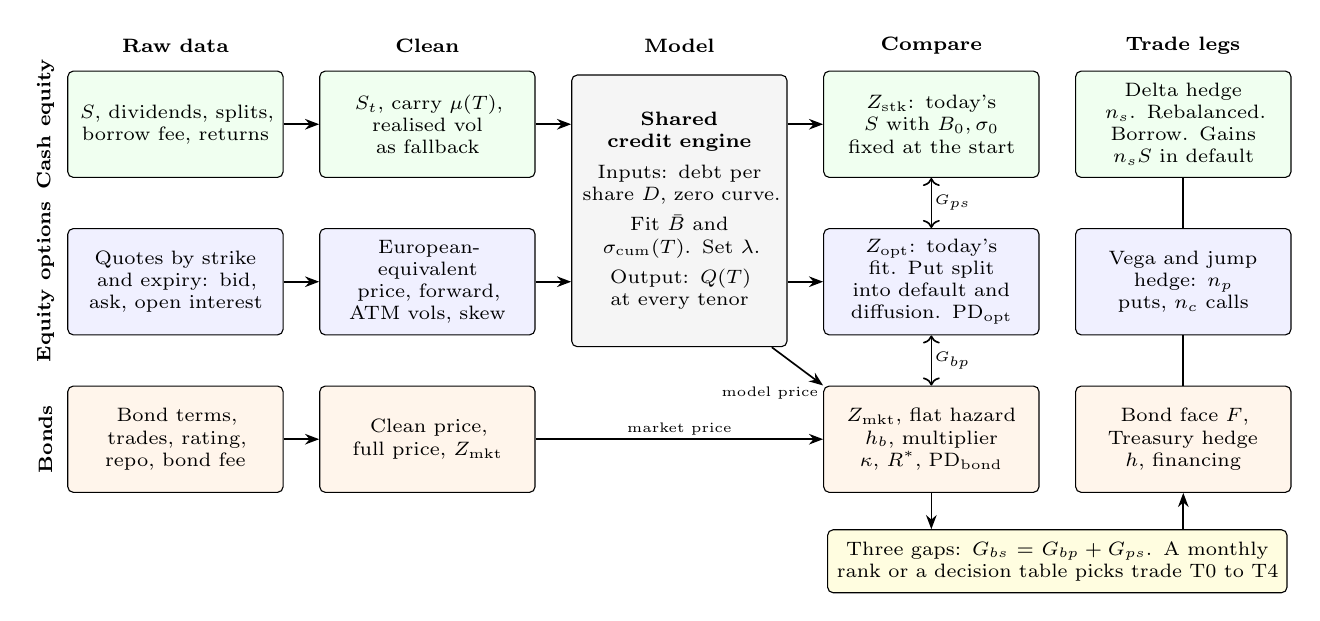
\begin{tikzpicture}[
  box/.style={draw,rounded corners=2pt,align=center,font=\scriptsize,minimum height=1.35cm,text width=2.5cm,fill=white},
  head/.style={font=\scriptsize\bfseries,align=center,text width=2.5cm},
  lane/.style={font=\scriptsize\bfseries,rotate=90,align=center},
  arr/.style={-{Stealth[length=1.8mm]},semithick},
  lab/.style={font=\tiny,fill=white,inner sep=1pt}]
\node[head] at (0,1.0) {Raw data};
\node[head] at (3.2,1.0) {Clean};
\node[head] at (6.4,1.0) {Model};
\node[head] at (9.6,1.0) {Compare};
\node[head] at (12.8,1.0) {Trade legs};
\node[lane] at (-1.65,0) {Cash equity};
\node[lane] at (-1.65,-2) {Equity options};
\node[lane] at (-1.65,-4) {Bonds};
\node[box,fill=green!6] (e1) at (0,0) {$S$, dividends, splits, borrow fee, returns};
\node[box,fill=green!6] (e2) at (3.2,0) {$S_t$, carry $\mu(T)$, realised vol as fallback};
\node[box,fill=blue!6] (o1) at (0,-2) {Quotes by strike and expiry: bid, ask, open interest};
\node[box,fill=blue!6] (o2) at (3.2,-2) {European-equivalent price, forward, ATM vols, skew};
\node[box,fill=orange!8] (b1) at (0,-4) {Bond terms, trades, rating, repo, bond fee};
\node[box,fill=orange!8] (b2) at (3.2,-4) {Clean price, full price, $\Zm$};
\node[box,minimum height=3.45cm,fill=gray!8] (m) at (6.4,-1.1) {\textbf{Shared credit engine}\\[3pt] Inputs: debt per share $D$, zero curve.\\[3pt] Fit $\Bbar$ and $\scum(T)$. Set $\lambda$.\\[3pt] Output: $Q(T)$ at every tenor};
\node[box,fill=green!6] (e3) at (9.6,0) {$\Zs$: today's $S$ with $B_0,\sigma_0$ fixed at the start};
\node[box,fill=blue!6] (o3) at (9.6,-2) {$\Zo$: today's fit. Put split into default and diffusion. $\PDopt$};
\node[box,fill=orange!8] (b3) at (9.6,-4) {$\Zm$, flat hazard $h_b$, multiplier $\kappa$, $R^*$, $\PDbond$};
\node[box,fill=green!6] (e4) at (12.8,0) {Delta hedge $n_s$. Rebalanced. Borrow. Gains $n_sS$ in default};
\node[box,fill=blue!6] (o4) at (12.8,-2) {Vega and jump hedge: $n_p$ puts, $n_c$ calls};
\node[box,fill=orange!8] (b4) at (12.8,-4) {Bond face $F$, Treasury hedge $h$, financing};
\node[box,minimum height=0.8cm,text width=5.6cm,fill=yellow!12] (g) at (11.2,-5.55) {Three gaps: $\Gbs=\Gbp+\Gps$. A monthly rank or a decision table picks trade T0 to T4};
\draw[arr] (e1)--(e2); \draw[arr] (o1)--(o2); \draw[arr] (b1)--(b2);
\draw[arr] (e2.east)--(m.west |- e2.east);
\draw[arr] (o2.east)--(m.west |- o2.east);
\draw[arr] (m.east |- e3.west)--(e3.west);
\draw[arr] (m.east |- o3.west)--(o3.west);
\draw[arr] (m.south east)++(-0.2,0)--(b3.north west); \node[lab] at (7.55,-3.42) {model price};
\draw[arr] (b2.east)--node[lab,above]{market price} (b3.west);
\draw[arr,<->] (e3)--node[lab,right]{$\Gps$} (o3);
\draw[arr,<->] (o3)--node[lab,right]{$\Gbp$} (b3);
\draw[arr] (b3.south)--(b3.south |- g.north);
\draw[arr] (b4.south |- g.north)--(b4.south);
\draw[semithick] (e4)--(o4); \draw[semithick] (o4)--(b4);
\end{tikzpicture}
\caption{How the three instruments connect. Read left to right. Options set the credit engine. The bond's price tests it. Stock and options hedge the result.}
\label{fig:pipeline}
\end{figure}

\begin{enumerate}[leftmargin=*,itemsep=2pt]
\item \textbf{Cash equity supplies $S$, carry and the delta hedge.} $S$ fixes the distance to the barrier through $V_0=S_0+B$. Realised vol is only a fallback here. The deck's vol is implied (slide 26).
\item \textbf{Equity options supply vol, skew and an implied default probability.} ATM vols by maturity bootstrap $\scum(T)$. The skew identifies $B$. A put contains a default part: the deck's 1.90 of 4.92 at the money, and 1.42 of 2.72 at 30\% out of the money.
\item \textbf{The credit engine turns those into $Q(T)$.} $Q$ prices any cash flow, so maturity mismatch between options and bonds disappears.
\item \textbf{Bonds supply the market credit spread, in place of CDS.} The deck does this itself on slide 14. The same $Q$ prices the bond's own cash flows and gives a model Z-spread to set against the market Z-spread.
\item \textbf{The gaps say which market is out of line.} With stock and fixed parameters on one side, and today's options on another, two gaps are independent (Section~\ref{sec:trades}).
\item \textbf{Greeks and jump to default come from the same model.} They size the stock, put and call legs (slides 20--25).
\item \textbf{Trades, P\&L, exits and reports are additions.} The deck has none of them.
\end{enumerate}

%-----------------------------------------------------------------------------
\section{Master table of raw inputs}\label{sec:inputs}

All names are neutral. ``Source'' is the instrument or data family, not a vendor. E, O, B, F and R label the groups used in Section~\ref{sec:steps}.

{\footnotesize
\begin{longtable}{@{}>{\raggedright\arraybackslash}p{2.35cm}>{\raggedright\arraybackslash}p{6.15cm}>{\raggedright\arraybackslash}p{1.5cm}>{\raggedright\arraybackslash}p{1.4cm}>{\raggedright\arraybackslash}p{1.6cm}>{\raggedright\arraybackslash}p{1.6cm}@{}}
\toprule
\textbf{Name} & \textbf{Meaning} & \textbf{Unit} & \textbf{Type} & \textbf{Frequency} & \textbf{Source}\\
\midrule\endhead
\multicolumn{6}{r}{\emph{continues}}\\\endfoot
\bottomrule\endlastfoot
E1 \fn{stock_close} & Closing share price & USD/share & float & daily & Cash equity\\
E2 \fn{split_factor} & Split and stock dividend adjustment & ratio & float & event & Cash equity\\
E3 \fn{dividend} & Cash dividend, by ex-date & USD/share & float & event & Cash equity\\
E4 \fn{shares_out} & Common shares outstanding & count & int & quarterly, event & Cash equity\\
E5 \fn{borrow_fee} & Stock loan fee & decimal/yr & float & daily & Cash equity\\
E6 \fn{hard_to_borrow} & Name flagged hard to borrow & flag & bool & daily & Cash equity\\
E7 \fn{stock_half_spread} & Half bid-ask on the stock & fraction & float & daily & Cash equity\\
E8 \fn{equity_id} & Issuer link to options and bonds & id & string & static & Cash equity\\
O1 \fn{option_id} & Underlying, expiry, strike, call or put & id & string & static & Options\\
O2 \fn{bid}, \fn{ask} & Closing option quotes & USD/share & float & daily & Options\\
O3 \fn{quote_time} & Time of the quote, to align with $S$ & time & time & daily & Options\\
O4 \fn{volume}, \fn{open_interest} & Liquidity of the contract & contracts & int & daily & Options\\
O5 \fn{exercise_style} & American or European & enum & enum & static & Options\\
O6 \fn{multiplier} & Contract size and any adjustment & shares & int & static & Options\\
O7 \fn{vendor_iv}, \fn{vendor_delta} & Optional cross-check only & decimal & float & daily & Options\\
B1 \fn{bond_id}, \fn{issuer_id} & Identifier and issuer link & id & string & static & Bonds\\
B2 \fn{coupon}, \fn{freq} & Coupon rate and payments a year & decimal, int & float, int & static & Bonds\\
B3 \fn{maturity}, \fn{issue_date} & Dates & date & date & static & Bonds\\
B4 \fn{day_count}, \fn{first_coupon} & Accrual conventions & enum, date & mixed & static & Bonds\\
B5 \fn{seniority} & Senior unsecured or other & enum & enum & static & Bonds\\
B6 \fn{call_schedule}, flags & Call dates and prices. Convertible, putable, sinking, floating flags & USD, flag & mixed & static & Bonds\\
B7 \fn{amount_out} & Face outstanding & USD mm & float & event & Bonds\\
B8 \fn{trade_price}, \fn{trade_size} & Each customer trade report & \% of par, USD & float & intraday & Bonds\\
B9 \fn{trade_time}, \fn{report_time} & Execution and publication time & time & time & intraday & Bonds\\
B10 \fn{side}, correction fields & Buy or sell. Reversal and correction links & enum & mixed & intraday & Bonds\\
B11 \fn{rating} & Rating known on the date & enum & enum & event & Bonds\\
B12 \fn{repo_rate}, \fn{bond_fee} & Financing of a long. Borrow cost of a short & decimal/yr & float & daily & Bonds\\
F1 \fn{st_debt}, \fn{lt_debt} & Short-term and long-term borrowings & USD mm & float & quarterly & Accounts\\
F2 \fn{other_st}, \fn{other_lt} & Other short-term and long-term liabilities & USD mm & float & quarterly & Accounts\\
F3 \fn{minority}, \fn{preferred} & Minority interest, preferred equity & USD mm & float & quarterly & Accounts\\
F4 \fn{total_liabilities} & For Yu's alternative $D$ & USD mm & float & quarterly & Accounts\\
F5 \fn{filing_time} & When each filing became public & time & time & quarterly & Accounts\\
R1 \fn{par_yields} & Treasury par yield by tenor & decimal & float & daily & Rates\\
R2 \fn{cash_rate} & Short rate for stock and option financing & decimal/yr & float & daily & Rates\\
R3 \fn{treasury_price} & Price of the Treasury used as hedge & USD/100 & float & daily & Rates\\
V1 \fn{events} & Merger, tender, call, default dates & date & date & event & Events\\
V2 \fn{realised_recovery} & Price after default, where known & \% of par & float & event & Events\\
V3 \fn{cds_par} & Optional. CDS par spread by tenor, as a check only & bp & float & daily & Credit, optional\\
\end{longtable}}

\textbf{Assumptions, not data.} $\Lbar$ (0.5 \DECK{9}), $\lambda$ (0.3 \LARDY\ \CG), $R_b$ (0.40), triggers, and the cost numbers. Section~\ref{sec:questions} ranks the choices.

%-----------------------------------------------------------------------------
\section{Every step}\label{sec:steps}

New code goes in \fn{fk_*.py} modules. \fn{e2c_bond.py} is imported, never edited. Its \fn{survival}, \fn{risky_bond_price}, \fn{default_leg} and \fn{run_bond_backtest} do not fit, because they assume one flat vol through \fn{Firm}. Its helpers below do fit. They price per 1 of face, and this plan's tables are per 100.

\subsection*{Stage A. Clean the market data}

\begin{step}{1}{equity_panel}{\ADAPT}
\item[Purpose] Build the daily stock series.
\item[Inputs] E1--E4, E8.
\item[Formula] Adjust $S$ for splits only. $x_t=\ln\big((S_t+\mathrm{div}_t)/S_{t-1}\big)$.
\item[Outputs] $S_t$, $\mathrm{div}_t$, $x_t$, shares. Used by 5, 7, 11, 12, 26, 32.
\item[Why] The deck takes $S$ as given. Corporate actions follow Yu's footnote 14 through \fn{debt_after_corporate_action}.
\end{step}

\begin{step}{2}{zero_curve_from_par_yields}{\ADAPT}
\item[Purpose] Build the discount curve. Reused from \fn{e2c_bond}.
\item[Inputs] R1.
\item[Formula] Bootstrap continuously compounded zeros.
\item[Outputs] \fn{ZeroCurve}, $\DF(t)$. Used by 4, 5, 14, 15, 16, 17.
\item[Why] The deck uses one flat rate. A bond needs each cash flow discounted at its own date. $Q(T)$ does not depend on the curve, so a full curve is allowed.
\end{step}

\begin{step}{3}{clean_option_quotes}{\ADAPT}
\item[Purpose] Remove quotes that cannot be priced.
\item[Inputs] O1--O6, $S_t$.
\item[Formula] Keep bid $>0$, ask $>$ bid, open interest $>0$, $(\text{ask}-\text{bid})/\text{mid}\le0.5$, expiry $\ge30$ days. Drop any quote that breaks: put price rises with $K$, convex in $K$, $P(K)/K$ rises with $K$.
\item[Outputs] Clean chain. Used by 4, 5, 6, 22.
\item[Why] Carr and Wu (2011, p.482) use bid $>0$ and open interest $>0$. The other bounds are my judgement.
\end{step}

\begin{step}{4}{european_equivalent}{\ADAPT}
\item[Purpose] Turn an American quote into a European price and a Black-Scholes vol.
\item[Inputs] Clean mids, $S_t$, curve, dividends, borrow fee.
\item[Formula] Solve $\mathrm{Tree}_{\mathrm{Am}}(v)=\text{mid}$ with discrete dividends. Then $P_E=\mathrm{BS}(v)$.
\item[Outputs] $P_E$, $\sigma_{BS}(K,T)$, $\Delta_{BS}$. Used by 5, 6, 8, 10, 22.
\item[Why] Listed single-stock options are American (Carr and Wu, p.481). The deck prices with Black-Scholes. The tree has no default, so it may understate the early-exercise value. WP8 measures that.
\end{step}

\begin{step}{5}{implied_forward}{\ADAPT}
\item[Purpose] Get the carry the option market actually uses.
\item[Inputs] $P_E$, $C_E$ near the money, $\DF(T)$.
\item[Formula] Regress $C_E-P_E=\DF(T)(F-K)$ across strikes. $\mu(T)=\ln(F/S)/T$.
\item[Outputs] $F(T)$, $\mu(T)$, an implied borrow estimate $r-p_{\mathrm{known}}-\mu$. Used by 8, 10, 16, 29.
\item[Why] Slide 4 calls $r$ a stock financing rate and $p$ a dividend yield. The forward bundles both, and it reveals a high borrow fee.
\end{step}

\begin{step}{6}{select_surface}{\DECK{8}\ \ADAPT}
\item[Purpose] Choose the points used for calibration.
\item[Inputs] $\sigma_{BS}(K,T)$, $\Delta_{BS}$, spreads, open interest.
\item[Formula] Maturities 0.5 years and longer. Strikes with $K/F\in[0.4,1.4]$. Out-of-the-money side only. Weight $w=1/$ half-spread in vol. Need 3 or more strikes below the money in 2 or more maturities for a skew fit.
\item[Outputs] Table of $(K,T,\sigma,w)$. Used by 8, 10.
\item[Why] The GX table spans $K/S$ of 0.48 to 1.43 at 1.59 and 2.59 years. The thresholds are my judgement. The deck has no rule.
\end{step}

\subsection*{Stage B. Calibrate the firm}

\begin{step}{7}{debt_per_share}{\YU\ \OWN}
\item[Purpose] Compute $D$. Reused from \fn{e2c_bond} for the default form.
\item[Inputs] F1--F5, E1, E4.
\item[Formula] Default: $D=$ total liabilities / shares. Variant: $\text{FinD}=\text{ST}+\text{LT}+0.5(\text{OtherST}+\text{OtherLT})$, $k_0=\min(\text{MI},0.5\,\text{FinD})$, $D=(\text{FinD}-k_0)/\big((\text{MktCap}+\text{Pref})/S\big)$. Use \fn{filing_usable_from} for timing.
\item[Outputs] $D_t$, both forms. Used by 9, 11, 13a, 25.
\item[Why] The deck says ``current debt per share'' with no formula (s.8, 9). Yu and Chen, Chen and Li (p.2015) both use total liabilities, so start there. The variant matches your master file on all 19,489 rows. $D$ matters more here than in Yu, because no spread fit absorbs its level.
\end{step}

\begin{step}{8}{fit_barrier_to_skew}{\DECK{8, 9, 11}\ \ADAPT}
\item[Purpose] Read the barrier from the skew, using one $B$ across maturities.
\item[Inputs] Step 6 table, $\mu(T)$, $\DF(T)$.
\item[Formula] $\min_{B,\sigma_1..\sigma_m}\sum_{i,j}w_{ij}\big(\sigma^{M}(K_i,T_j;B,\sigma_j)-\sigma_{ij}\big)^2$, with $\sigma^M$ from step 16.
\item[Outputs] $B_{\text{skew}}$, $\sigma_j$, rmse, status. Used by 9.
\item[Why] The deck uses ``the same default barrier level'' for two maturities and prints no objective. On GX market vols this returns $B=6.01$, against the deck's 6.
\end{step}

\begin{step}{9}{choose_barrier}{\DECK{9, 11}\ \ADAPT}
\item[Purpose] Pick the barrier to use.
\item[Inputs] $B_{\text{skew}}$, rmse, $D$, $\Lbar=0.5$.
\item[Formula] $\Bbar=\Lbar D$ by default. Use $B_{\text{skew}}$ only if it cuts rmse by 0.5 vol points or more, and $0.25D\le B_{\text{skew}}\le D$. Hold $\Bbar$ fixed until the next filing.
\item[Outputs] $\Bbar_t$, source flag. Used by 10, 12, 15, 16, 23.
\item[Why] The deck allows either route. $B$ is weakly identified: on GX, rmse stays within 0.23 vol points for $B$ from 5 to 7. The 2.59-year default probability moves by 0.026 over that range, so the error does little harm.
\end{step}

\begin{step}{10}{bootstrap_asset_vol}{\DECK{11, 12}\ \ADAPT}
\item[Purpose] Build the asset vol term structure.
\item[Inputs] ATM $\sigma_{BS}(T_j)$, $\Bbar$, $\mu(T)$.
\item[Formula] Solve $\sigma^M(F,T_j;\Bbar,\scum(T_j))=\sigma_{BS}(F,T_j)$. Total variance $v_j=\scum^2(T_j)T_j$. Forward variance $(v_j-v_{j-1})/(T_j-T_{j-1})$, which must be positive. Linear in total variance between maturities. Flat forward past the last one.
\item[Outputs] $\scum(T)$ and the forward vols. Used by 12, 13, 16.
\item[Why] Slide 12 says ``boot-strapped'' and stops there. Solving the model beats the slide 6 rule: at GX the rule gives 52.3\%, against the deck's 49.8\%. The GX forward is 40.7\%. With it the slide 12 curve reproduces within 17 bp.
\end{step}

\begin{step}{11}{asset_vol_fallback}{\OWN\ \CG}
\item[Purpose] Give a vol when a name has no usable options.
\item[Inputs] $x_t$, $S$, $\Bbar$.
\item[Formula] $\sigma=\sigma_S\,S/(S+\Bbar)$. $\sigma_S$ is the mean of 30, 60, 90, 180 and 360 day realised vols. Reuse \fn{historical_equity_vol} per window. Variant for step 13a: 3-year daily $\sigma_S$, then $\sigma=\sigma_S(1-R_0)f$ with $R_0=D/(S+D)$ and $f=$ 1, 1.05, 1.10, 1.20, 1.40, 1.80 at breaks 0.25, 0.35, 0.45, 0.55, 0.75.
\item[Outputs] Flat $\scum$, flagged as fallback. Used by 12.
\item[Why] The deck has no fallback. In the rerun of your workbooks the realised blend gave Sharpe 2.49, and 162-week vol gave 0.15. CreditGrades and Yu use 1,000 days. The two own-file numbers are gross and in-sample. The variant is the rule in Chen, Chen and Li (p.2015). It gives $0.60\sigma_S$ against CreditGrades' $0.67\sigma_S$ at $S/D=1$, and $0.36\sigma_S$ against $0.33\sigma_S$ at $S/D=0.25$.
\end{step}

\subsection*{Stage C. Survival curve}

\begin{step}{12}{fk_survival}{\DECK{11, 18}}
\item[Purpose] Survival probability at one tenor.
\item[Inputs] $T$, $S_0$, $\Bbar$, $\scum(T)$, $\lambda$.
\item[Formula] $Q(T)=N\!\big(\tfrac{\ln\dbar}{A_T}-\tfrac{A_T}{2}\big)-\dbar\,N\!\big(\!-\tfrac{\ln\dbar}{A_T}-\tfrac{A_T}{2}\big)$, with $A_T=\sqrt{\scum^2(T)T+\lambda^2}$ and $\dbar=\tfrac{S_0+\Bbar}{\Bbar}e^{\lambda^2}$. At $\lambda=0$ this is slide 11.
\item[Outputs] $Q(T)$. Used by 13.
\end{step}

\begin{step}{13}{fk_curve}{\DECK{19}}
\item[Purpose] Survival on a grid, with the short-end remedy.
\item[Inputs] Step 12 at $T\ge0.5$.
\item[Formula] For $T<0.5$ and $\lambda>0$: $Q(T)=Q(0.5)^{T/0.5}$, which is flat intensity from 1. Grid of 1/48 year.
\item[Outputs] $Q$ on the grid. Hazard $h(T)$. Used by 14, 15, 19--23.
\end{step}

\begin{step}{13a}{des_survival}{\ADAPT}
\item[Purpose] Survival in the extended CreditGrades model, to replicate the published gap.
\item[Inputs] $V_0=S_0+\Lbar D$, $\Lbar=0.5$, $\lambda=0.3$, $\sigma$ from step 11 variant, $r$, payout $\delta$.
\item[Formula] $q(t)=\int_{-\infty}^{\bar z}q(t|z)\phi(z)\,dz$, $\bar z=\tfrac{\lambda}{2}-\tfrac1\lambda\ln\tfrac{\Lbar D}{V_0}$. $q(t|z)=N\big(C\sigma\sqrt t-\tfrac{y}{\sigma\sqrt t}\big)-e^{2Cy}N\big(C\sigma\sqrt t+\tfrac{y}{\sigma\sqrt t}\big)$, with $C=\tfrac{r-\delta}{\sigma^2}-\tfrac12$ and $y=-\ln\tfrac{V_0}{\Lbar D}-\tfrac{\lambda^2}{2}+\lambda z$. $\delta=$ (dividends + interest + repurchases)/$(S+D)$, capped at 0.15.
\item[Outputs] $q(t)$. Used by 15, 23, 24a.
\item[Why] This is Chen, Chen and Li (Eqs.\ 1--9, pp.2012--2014). It differs from slide 18 in two ways: $V$ drifts at $r-\delta$, and barriers above $V_0$ are cut off. At zero drift and $T=1$ it gives 0.936004 against Eq.\ (1)'s 0.934494 at $S/\Bbar=1$. Keep the deck's zero-drift form for all option work.
\end{step}

\subsection*{Stage D. Model values}

\begin{step}{14}{fk_cds}{\DECK{12}\ \LARDY\ \CG}
\item[Purpose] CDS legs and par spread, for tests and for sizing.
\item[Inputs] $Q$, $\DF$, $R$, premium frequency.
\item[Formula] $L=\sum_j\DF(\text{mid}_j)(Q_{j-1}-Q_j)$. $A=\sum_i\Delta_i\DF(t_i)Q(t_i)+\tfrac12\Delta L$. Par $=(1-R)L/A$. Optional $\times360/365$ (CreditGrades, printed p.9).
\item[Outputs] $A$, $L$, par. Used by 26, 31.
\item[Why] The deck prints no CDS formula. Lardy's printed slide 7 gives the integral form. Deck charts fit it at $r=5\%$.
\end{step}

\begin{step}{15}{fk_bond_price}{\DECK{12}\ \ADAPT}
\item[Purpose] Value this bond's own cash flows on the model curve.
\item[Inputs] Bond terms, $Q$, $\DF$, $R_b$. \fn{cash_flows} from \fn{e2c_bond}.
\item[Formula] $P=\sum_i CF_i\,\DF(t_i)\,Q(t_i)+R_b\,L(T)$, then $Z$ from \fn{z_spread}.
\item[Outputs] $P_{\text{opt}},\Zo$ and, with step 23's curve, $P_{\text{stk}},\Zs$. Used by 24, 26.
\item[Why] Slide 12 says it computes bond prices and prints no formula. This is the form of \fn{risky_bond_price}. Recovery is of par, so a discount bond loses less than a premium bond. With flat 42\% vol at $r=5\%$ it gives clean prices 83.4, 59.9, 44.5 against the deck's 82, 60, 43.
\end{step}

\begin{step}{16}{fk_put}{\DECK{1, 6}\ \ADAPT}
\item[Purpose] Price a put and split it into default and diffusion parts.
\item[Inputs] $S_0,K,T,\scum(T),B,r,p$.
\item[Formula] At $\lambda=0$: default part $=K\,e^{-rT}(1-Q(T))$. Diffusion part $=e^{-pT}\big[G(V_0)-\tfrac{V_0}{B}G(B^2/V_0)\big]$, where $H=B+Ke^{-(r-p)T}$ and $G(x)=H[N(-d_2(x,H))-N(-d_2(x,B))]-x[N(-d_1(x,H))-N(-d_1(x,B))]$. $d_1(x,y)=\big(\ln(x/y)+\tfrac12\scum^2T\big)/(\scum\sqrt T)$, $d_2=d_1-\scum\sqrt T$. Call by parity. Invert for $\sigma^M$.
\item[Outputs] Put, default part, diffusion part, $\sigma^M(K,T)$. Used by 8, 10, 22, 26.
\item[Why] Slide 6 says closed form and prints none. This is the reflection principle. It reproduces slide 8 within 0.14 vol points and matches direct integration to 8 decimals.
\end{step}

\subsection*{Stage E. Market side and gaps}

\begin{step}{17}{market_z}{\ADAPT}
\item[Purpose] Get the market spread of the bond.
\item[Inputs] B1--B10, $\DF$.
\item[Formula] Reuse \fn{clean_trade_reports}, \fn{fix_decimal_shifts}, \fn{flag_price_spikes}, \fn{daily_clean_price}, \fn{full_price}, \fn{z_spread}. Screen with \fn{bond_terms_are_eligible}, \fn{maturity_is_eligible}, \fn{passes_liquidity_screen}.
\item[Outputs] Full price, $\Zm$. Used by 18--21, 24.
\item[Why] This is Part 3 of \fn{notes/paper_method/02_bond_vol_method.md}. Z against Z compares like with like on one bond's cash flows.
\end{step}

\begin{step}{18}{bond_implied_curve}{\DECK{14}\ \ADAPT}
\item[Purpose] Turn one bond into a market credit curve, as slide 14 does.
\item[Inputs] Full price, bond terms, $\DF$, $R_b$.
\item[Formula] Solve $\sum_iCF_i\DF(t_i)e^{-ht_i}+R_b\int_0^{T}\DF(s)he^{-hs}ds=P$. Bond-implied par $s_b=(1-R_b)h_b$.
\item[Outputs] $h_b$, $s_b$. Used by 30 and test C4.
\item[Why] Slide 14 gives the idea and no procedure. A flat hazard is the simplest reading. On 10/1/01 it gives 30.7\% to 38.3\% (price as clean or full), against about 31\% on the chart.
\end{step}

\begin{step}{19}{hazard_multiplier}{\ADAPT}
\item[Purpose] Compare a bond and an option at the same horizon.
\item[Inputs] $Q$, full price, $R_b$.
\item[Formula] Solve $\kappa$ so that $Q^\kappa$ prices the bond. $\PDbond(T)=1-Q(T)^\kappa$.
\item[Outputs] $\kappa$, $\PDbond(T)$. Used by 30.
\item[Why] One bond cannot give a curve. The model's shape carries the bond's level to the option's maturity. Chan et al. (2023, p.190) show maturity mismatch matters. $\kappa>1$ means the bond is wider than options imply.
\end{step}

\begin{step}{20}{implied_recovery}{\ADAPT}
\item[Purpose] Ask what recovery would close the gap.
\item[Inputs] $Q$, full price.
\item[Formula] Solve $R^*$ so that step 15 equals the full price. Flat form: use hazard $\lambda_p$ from step 22 in step 18's price, and solve for $R^*$.
\item[Outputs] $R^*$, flag if outside $[0,0.8]$. Used by 30.
\item[Why] Slide 20 calls recovery ``a big assumption''. B\'egin et al. (2023, pp.123, 125) extract recovery from put-implied intensity and CDS as $R=1-\mathrm{CDS}/\lambda$. This is the same idea on a bond. They find under 1\% of values negative (p.126, note 4). The bounds here are my judgement.
\end{step}

\begin{step}{21}{bond_implied_vol}{\ADAPT}
\item[Purpose] Express the bond's spread in vol units.
\item[Inputs] $\scum(\cdot)$, $\Bbar$, full price, $R_b$.
\item[Formula] Solve $c$ so that $\scum(\cdot)\to c\,\scum(\cdot)$ prices the bond. Scan for all roots. Use the status codes of \fn{implied_vol_bond}.
\item[Outputs] $c$, status. Used by 30.
\item[Why] CreditGrades (p.13) and Yu (PDF p.10) define this for CDS. \fn{implied_vol_bond} assumes flat vol, so it needs a scale on the curve. A bond can have two roots near recovery.
\end{step}

\begin{step}{22}{option_implied_default}{\DECK{11}\ \ADAPT}
\item[Purpose] Extract default probability from puts in two ways.
\item[Inputs] Step 13, American mids, $\Delta_{BS}$, $\DF$.
\item[Formula] Model route: $\PDopt(T)=1-Q(T)$. Model-free route: take the lowest strike with $|\Delta|\le0.15$ and mid $\ge0.15$. $U_p=P_A(K)/K$. Solve $U_p=\lambda_p(1-e^{-(r+\lambda_p)T})/(r+\lambda_p)$. $\mathrm{PD}_p=1-e^{-\lambda_pT}$.
\item[Outputs] $\PDopt(T)$, $U_p$, $\lambda_p$, $\mathrm{PD}_p$. Used by 30.
\item[Why] The model-free route is Carr and Wu (2011, Eqs.\ 1, 4, pp.479--480). It assumes a default corridor, and Finkelstein's model has none (see Section~\ref{sec:options}). The gap between the two routes measures that.
\end{step}

\begin{step}{23}{stock_only_curve}{\DECK{12, 13, 14, 15}\ \ADAPT}
\item[Purpose] Compute the model the stock alone implies, with parameters held fixed.
\item[Inputs] $B_0=\Bbar$ and flat $\sigma_0=\scum(1)$ fixed on a start date, $S_t$. Refit every 250 trading days. Variant: step 13a with rolling 3-year vol, which needs no options.
\item[Formula] $Q$ from step 13 with today's $S_t$, then step 15.
\item[Outputs] $\Zs$. Used by 24.
\item[Why] This is the deck's own test design: ``Using the same model parameters for different dates'' (s.12), $B=6$, $\sigma=42\%$ held for 15 months (s.13). The 250-day refit is my judgement.
\end{step}

\begin{step}{24}{three_gaps}{\ADAPT}
\item[Purpose] Measure the three gaps.
\item[Inputs] $\Zm,\Zo,\Zs$. \fn{log_gap}.
\item[Formula] $\Gbp=\ln(\Zm/\Zo)$. $\Gps=\ln(\Zo/\Zs)$. $\Gbs=\ln(\Zm/\Zs)=\Gbp+\Gps$.
\item[Outputs] Three gaps per bond per day. Used by 25, 30, 33.
\item[Why] Slide 26 speaks of one residual. Three markets give two independent ones, and the pair tells which market moved. A positive gap means the first market is wider.
\end{step}

\begin{step}{24a}{des_gap}{\ADAPT}
\item[Purpose] Compute the published bond-against-stock gap and rank it.
\item[Inputs] Step 13a in step 15, recovery $\alpha\Lbar=0.35$, market full price, lagged bond value.
\item[Formula] $\mathrm{DES}=CS_D-CS_E$ in bp per bond. Each spread is the bond yield less the yield of a synthetic Treasury with the same cash flows. Average to the firm with lagged bond value as weight. Sort firms into quintiles each month. Accounting data lag at least 2 months.
\item[Outputs] DES, firm and bond level, quintile. Used by 30, 34.
\item[Why] This is Chen, Chen and Li (pp.2015--2016). It is $\Zm-\Zs$ in levels, up to the choice of spread. Their typical quintile values are $-139$, $+45$, $+103$, $+156$ and $+271$ bp (p.2023). Note the middle firm has a gap of $+103$ bp, not zero.
\end{step}

\begin{step}{24b}{impvol_change}{\ADAPT}
\item[Purpose] Measure the monthly rise in 1-year implied vol.
\item[Inputs] Month-end ATM call and put implied vol, interpolated to 365 days.
\item[Formula] $\Delta\text{ImpVOL}_t=\tfrac12(\Delta\text{CVOL}_t+\Delta\text{PVOL}_t)$. Rank into deciles each month.
\item[Outputs] $\Delta$ImpVOL, decile. Used by 30.
\item[Why] This is Cao et al.\ (2023, pp.1375--1376, 1379). It uses options the bond has not yet priced. It is the time-series counterpart of a rising $\Gps$.
\end{step}

\begin{step}{25}{control_gaps}{\ADAPT\ \OWN}
\item[Purpose] Take out liquidity and common moves.
\item[Inputs] Gaps, peers, sibling, illiquidity fields, $S/D$.
\item[Formula] (1) Subtract \fn{peer_median_gap}. (2) Require \fn{sibling_confirms}. (3) Own-files variant: each week regress $\ln c$ on $\ln(S/D)$ across names, and keep the residual. (4) Variant: regress the gap on bid-ask, log size and age. Check VIF first, since these fields correlate. (5) Variant from your basis note: regress on credit index and swap spread, fit a mean-reverting model to the residual, and use the simulated expected capture as the signal.
\item[Outputs] Adjusted gaps. Used by 30.
\item[Why] The model has no input for supply, demand or the basis (CreditGrades p.32). Most investment-grade spread is not credit risk (literature review, line 81). The own-files agent reads the cross-section's free intercept as absorbing an average bond premium. Nothing has tested that on bonds. Chen, Chen and Li find the bond premium survives illiquidity and jump controls (p.2031), so controls may not remove all of it. Variant (5) is from the scanned \emph{3 Steps of CDS Bond Basis}, which has no stated author and is for a CDS basis.
\end{step}

\subsection*{Stage F. Risk}

\begin{step}{26}{fk_greeks}{\DECK{20}\ \ADAPT}
\item[Purpose] Compute delta, gamma, vega and jump to default per instrument.
\item[Inputs] Steps 14, 15, 16. Position.
\item[Formula] $\delta$, $\gamma$: bump $S$ by $\pm1\%$, holding $\scum(\cdot)$, $\Bbar$, $\lambda$. $\nu$: scale $\scum(\cdot)$ by $1\pm0.001$. Jump $J$: bond $-(P-100R_b)$, CDS seller $-100(1-R)$, put $Ke^{-rT}-\text{Put}$, stock $-S$, call $-\text{Call}$.
\item[Outputs] $(\delta,\gamma,\nu,J)$ per unit, and the put-only ratio $-\delta_P/\delta_p$. Used by 27, 28, 29, 31.
\item[Why] Slide 20 names the sensitivities and does not define them. Asset vol held fixed gives $-26.9$ on slide 21 against about $-27.4$. Equity vol held fixed gives $-11.1$. So the deck holds asset vol fixed. Leaving contract value out of the CDS jump fits slides 23--25 best. The put-only ratio follows Avino and Salvador (p.10), who hedge market value through the common state variable. Here $\partial/\partial V=\partial/\partial S$.
\end{step}

\begin{step}{27}{solve_hedge}{\DECK{21, 22, 23, 24}}
\item[Purpose] Solve the hedge amounts.
\item[Inputs] Target greeks $g$, instrument greeks $M$.
\item[Formula] Solve $M\,n=-g$. Delta only: stock, or put alone. Delta and vega: put and stock. Delta and jump: put and stock. All three: put, stock, call. Guards \ADAPT: reject if a put or call count is negative, or the stock dollar size exceeds 1.5 times the bond's value. Report the condition number, but do not filter on it.
\item[Outputs] $n=(n_p,n_s,n_c)$, status. Used by 31.
\item[Why] The guards are mine. The solve can fail. On GX with a 7.5 put and a 15 call it returns $-12.7$ puts and $-\$192$ of stock. The condition number cannot separate good from bad, since it is 759 here and 509 on the deck's own slide 24.
\end{step}

\begin{step}{28}{optimal_strike}{\DECK{25}}
\item[Purpose] Use one put plus stock for all three exposures.
\item[Inputs] Steps 16, 26.
\item[Formula] Find $K^*$ where the delta and vega solution also zeroes jump: $n(K)\,J_p(K)-n_s(K)S+g_J=0$.
\item[Outputs] $K^*$, $n_p$, $n_s$. Used by 31.
\item[Why] Slide 25 gives $K^*=39.2$ and no definition. This reading gives 39.5.
\end{step}

\begin{step}{29}{rehedge_due}{\DECK{20}\ \ADAPT}
\item[Purpose] Decide when to rebalance.
\item[Inputs] Held and target shares, days since last, $S$ move, costs.
\item[Formula] Rebalance weekly, or if $|n_{\text{target}}/n_{\text{held}}-1|>10\%$. Compare with static \YU\ and weekly \OWN.
\item[Outputs] Flag. Used by 32.
\item[Why] Slide 20 says ``not static'' and sets no rule. Yu finds daily rebalancing does not help. Your master file refreshes weekly. The 10\% is my judgement.
\end{step}

\subsection*{Stage G. Trades. Everything here is an addition to the deck}

\begin{step}{30}{decide_trade}{\ADAPT\ \YU}
\item[Purpose] Turn gaps into one action.
\item[Inputs] Ranks, adjusted gaps, $\Delta$ImpVOL, $\kappa$, $R^*$, status flags, costs.
\item[Formula] Base: the monthly rank in step 24a. Top quintile is long bond, short stock. Bottom quintile is the reverse. Skip a long-bond entry if $\Delta$ImpVOL is in the top decile. Name-by-name variant: Table~\ref{tab:decide}, with trigger $g$ starting at $\ln1.5=0.405$, in \fn{peer_adjusted_signal}. Also \fn{passes_cost_gate}, \fn{sibling_confirms}, \fn{vol_status_allows_trade}. Trade at \fn{execution_day} with lag 1.
\item[Outputs] Trade type and side. Used by 31.
\item[Why] A rank has the published evidence, and it does not need a zero-mean gap. A fixed ratio test is biased at a fixed $\Lbar$. In Chen, Chen and Li's middle quintile, $\ln(151.5/46.8)=1.17$, well past 0.405 (p.2023). Yu's per-name fit of $\Lbar$ removes that level. Trading the next day guards against price error entering both signal and return (paper\_method Step 35). The $\Delta$ImpVOL skip is my addition.
\end{step}

\begin{step}{31}{size_trade}{\ADAPT\ \YU\ \OWN}
\item[Purpose] Size each leg.
\item[Inputs] Greeks, \fn{cds_equivalent_face}, \fn{rate_hedge_face}.
\item[Formula] Rank book: equal or lagged-value weight within a quintile, each leg to the same gross. Name-by-name: $F=A_{5y}/D_b$, then $n$ from step 27, and $h=F\cdot$\fn{rate_hedge_face}. Variant \OWN: size so that a 3 vol point convergence earns a set amount, capped.
\item[Outputs] $F,n_s,n_p,n_c,h$. Used by 32.
\item[Why] This keeps Yu's capital of 0.5 per unit of 5-year spread risk meaningful. Your master file sizes by target P\&L over vega. The per-name cap there is \$10mm.
\end{step}

\begin{step}{32}{leg_pnl}{\ADAPT}
\item[Purpose] Compute daily P\&L per leg.
\item[Inputs] Sizes, marks, carry.
\item[Formula] Section~\ref{sec:trades}. \fn{daily_pnl} covers T1. T2 to T4 need signed stock and option legs, because \fn{daily_pnl} ties the stock's sign to the bond's.
\item[Outputs] P\&L per leg, account value by \fn{next_account_value}. Used by 33, 34.
\end{step}

\begin{step}{33}{exit_rule}{\YU\ \ADAPT}
\item[Purpose] End the trade.
\item[Inputs] Gaps, days held, value, events, option expiry.
\item[Formula] Rank book: rebalance monthly. Test holding 1, 3 and 6 months. Otherwise \fn{bond_exit_reason}, plus: option within 30 days of expiry (roll or close), and gap sign flip on $\Gbp$ for T2 and T4.
\item[Outputs] Exit reason. Used by 34.
\item[Why] Chen, Chen and Li find bond returns lose significance by month 3, and are near zero after a year (p.2035). The quintile gap is still above 200 bp two years on (p.2033). So a convergence exit will rarely fire, as in Yu's Table 3.
\end{step}

\begin{step}{34}{book_and_report}{\YU\ \OWN}
\item[Purpose] Aggregate and report.
\item[Inputs] Closed trades, daily returns.
\item[Formula] \fn{monthly_index}, \fn{annual_sharpe}, \fn{trade_summary}, \fn{monthly_summary}, \fn{attribute_pnl}, \fn{break_even_cost} and \fn{lag_sensitivity}. Report by trade type, direction, rating at entry. Also report capital from single-name default stress, as in your master file. If you test a grid of entry and exit rules, report the probability of backtest overfitting and the deflated Sharpe, as in your scanned basis note.
\item[Outputs] Section~\ref{sec:outputs}.
\end{step}

%-----------------------------------------------------------------------------
\section{Master table of final outputs}\label{sec:outputs}

{\footnotesize
\begin{longtable}{@{}>{\raggedright\arraybackslash}p{3.0cm}>{\raggedright\arraybackslash}p{6.9cm}>{\raggedright\arraybackslash}p{1.7cm}>{\raggedright\arraybackslash}p{1.3cm}>{\raggedright\arraybackslash}p{2.1cm}@{}}
\toprule
\textbf{Output} & \textbf{Meaning} & \textbf{Unit} & \textbf{Step} & \textbf{Frequency}\\
\midrule\endhead
\multicolumn{5}{r}{\emph{continues}}\\\endfoot
\bottomrule\endlastfoot
$\Bbar$, source flag & Barrier and how it was set & USD/share & 9 & per filing\\
$\scum(T)$, forward vols & Asset vol term structure & decimal & 10 & daily\\
$Q(T)$, $h(T)$ & Survival curve and hazard & decimal & 13 & daily\\
Model par spread & CDS-equivalent on the model curve & bp & 14 & daily\\
$P_{\text{opt}},\Zo$ & Bond value and spread on today's options & USD/100, bp & 15 & daily\\
$P_{\text{stk}},\Zs$ & Same, on fixed parameters and today's $S$ & USD/100, bp & 23 & daily\\
Put default part & $Ke^{-rT}(1-Q)$ by strike and maturity & USD/share & 16 & daily\\
Put diffusion part & The rest of the put & USD/share & 16 & daily\\
Default share & Default part over put price & decimal & 16 & daily\\
$\sigma^M(K,T)$ & Model Black-Scholes vol, for skew comparison & decimal & 16 & daily\\
$\Zm$, full price & Market spread and price & bp, USD/100 & 17 & daily\\
$h_b$, $s_b$ & Flat bond hazard, bond-implied par spread & decimal, bp & 18 & daily\\
$\kappa$, $\PDbond(T)$ & Hazard multiplier, bond default probability & decimal & 19 & daily\\
$R^*$ & Recovery that closes the bond gap & decimal & 20 & daily\\
$c$, status & Bond-implied scale on asset vol & ratio & 21 & daily\\
$\PDopt(T)$, $U_p$, $\mathrm{PD}_p$ & Option default probability, model and model-free & decimal & 22 & daily\\
$\Gbp,\Gps,\Gbs$ & The three log gaps, raw and adjusted & log ratio & 24, 25 & daily\\
DES, quintile & Published level gap, bond and firm & bp, rank & 24a & monthly\\
$\Delta$ImpVOL, decile & Monthly rise in 1-year ATM vol & decimal, rank & 24b & monthly\\
$(\delta,\gamma,\nu,J)$ & Greeks and jump per instrument and position & per unit & 26 & daily\\
$n$, status, $K^*$ & Hedge amounts, including put-only, and optimal strike & count & 27, 28 & at trade\\
Trade log & Type, side, dates, sizes, exit reason, P\&L per leg & USD & 30--33 & per trade\\
Account value, return & Net of financing and costs & USD, decimal & 32 & daily\\
Monthly index & Compounded returns by trade type & decimal & 34 & monthly\\
Sharpe, $t$, drawdown & Annualised, net and gross, by group & number & 34 & per run\\
Attribution & Bond, stock, option, Treasury, financing, cost & USD & 34 & per run\\
Break-even cost & Cost multiple that takes the Sharpe to zero & multiple & 34 & per run\\
Empirical hedge slope & Stock beta of the rate-hedged bond, against model delta & number & 34 & per run\\
\end{longtable}}

%-----------------------------------------------------------------------------
\section{How to do each leg}\label{sec:legs}

\subsection{Bonds}\label{sec:bonds}

\textbf{Which spread: Z-spread over the Treasury zero curve.} It uses the bond's own cash flows and the whole curve, and the model can produce the same number by the same solver. Reasons and alternatives are in Part 3 of \fn{02_bond_vol_method.md}. Compare Z only with Z. A bond's Z differs from a CDS spread for arithmetic reasons once the bond is away from par. In that note's example, the 5-year CDS is 167.6 bp while model Z runs from 155.9 bp at a 2\% coupon to 177.0 bp at 9\%.

\textbf{Run the matched-Treasury spread as a check.} Chen, Chen and Li use the bond yield less the yield of a synthetic Treasury with the same cash flows (pp.2015--2016). Their replication needs that form. Z-spread stays the base for name-by-name work, because the model and market use the same solver.

\textbf{Keep the deck's bond-implied CDS as a second measure.} Step 18 repeats slide 14. It lets you compare with the deck's charts and with any CDS you later obtain.

\textbf{Turning the survival curve into a value for this bond.} Use step 15. Each coupon and the principal count only if the firm survives to that date. Recovery pays at default. The $\kappa$, $R^*$ and $c$ of steps 19--21 restate the same price gap in hazard, recovery and vol units. On GX they are 0.908, 0.356 and 0.953 (Appendix~\ref{app:gx}).

\textbf{Recovery.}
\begin{enumerate}[nosep]
\item Use recovery of par, $R_b=0.40$, for senior unsecured. A claim in bankruptcy is on par, not on market price.
\item Run the deck's values as sensitivities. Slide 14 shows the effect at GX's peak: R of 0.30 gives a model par near 37\%, and R of 0.10 gives near 47.5\%.
\item Use 0.35 in the published replication. Chen, Chen and Li set $\alpha=0.7$ with $\Lbar=0.5$ (p.2015).
\item Keep $R_b$ apart from $\Lbar$. $\Lbar$ is recovery on all liabilities and sets the barrier. $R_b$ is recovery on this issue (Yu, PDF p.35).
\item Flag any $R^*$ outside $[0,0.8]$. That points to a wrong curve or a non-default premium, not to a real recovery.
\end{enumerate}

\textbf{Illiquidity and basis control.} The model has no inputs for bond supply, demand or the basis (CreditGrades p.32). So:
\begin{enumerate}[nosep]
\item Trade high yield first. Lardy's printed slide 25 shows correlation of spread changes rising with risk: 0.10 for AA, 0.32 for BBB, 0.50 for BB and 0.72 for B. Your literature review says most investment-grade spread is not credit risk (line 81).
\item Subtract the peer median each day, by rating and maturity bucket (step 25).
\item Require the sibling bond to agree (step 25).
\item Run the own-files cross-section as a variant. Nothing has tested it on bonds. The original plan named it: ``analysis of residuals in price term p(mkt) $-$ p(EVol) allows to include securities other than CDS'' (\fn{03_bond_and_vol.md}).
\item Use CDS as a check if it exists, through \fn{cds_confirms}. Kim, Li and Zhang (2016) find the residual basis predicts bond returns (1.79\% at 20 days). So a bond-only gap may be a basis trade, not an equity-credit one.
\item Expect the premium to sit where costs are highest. Chen, Chen and Li report $-2.69\%$ a year for large bonds against $-6.16\%$ for small ones (p.2037). So report results by bond size, and trust the large-bond number.
\end{enumerate}

\textbf{Callable bonds.} High yield names often have only callable bonds. Part 1 of the note keeps one only if it trades 5 points or more under the next call price, valued to maturity. Measure how many names survive that screen before relying on it.

\textbf{Reuse from \fn{e2c_bond.py}.} All of Part 1 screens, price cleaning, Z solver, duration, Treasury hedge, financing, costs and exits. \textbf{Do not reuse} \fn{survival}, \fn{risky_bond_price}, \fn{bond_equity_delta} or \fn{run_bond_backtest}, since they assume one flat vol. Add a test that \fn{fk_bond_price} matches \fn{risky_bond_price} at flat vol with the remedy off.

\subsection{Options}\label{sec:options}

\textbf{Decomposing a put.} Step 16 gives the split. Default pays the strike, since the stock goes to zero (slide 1). The rest is a knock-out put on $V$. The default share falls as the strike rises and grows with maturity:

\begin{center}
\footnotesize
\begin{tabular}{@{}rrrrrrr@{}}
\toprule
\textbf{Strike} & \textbf{Put, 2.59y} & \textbf{Default part} & \textbf{Diffusion part} & \textbf{Default share} & \textbf{Share, 1.59y} & \textbf{BS vol, 2.59y}\\
\midrule
5 & 1.485 & 1.231 & 0.253 & 0.829 & 0.700 & 91.6\%\\
7.5 & 2.515 & 1.847 & 0.668 & 0.734 & 0.570 & 83.5\%\\
10 & 3.735 & 2.463 & 1.272 & 0.659 & 0.482 & 78.4\%\\
12.5 & 5.118 & 3.078 & 2.040 & 0.601 & 0.421 & 75.0\%\\
15 & 6.637 & 3.694 & 2.943 & 0.557 & 0.377 & 72.4\%\\
\bottomrule
\end{tabular}

\smallskip
GX on 6/14/01. $S=10.5$, $B=6$, $r=5\%$. Asset vol 46.5\% to 2.59y and 49.8\% to 1.59y. All from the deck's parameters.
\end{center}

This means a low-strike put is mostly a credit instrument, and an at-the-money long-dated put is still more than half credit on this name. The deck's slide 1 makes the same point at 0.386 and 0.522 of the put. Its two figures do not follow one formula (Section~\ref{sec:tests}).

\textbf{Extracting default probability.} Use two routes, and report both.
\begin{enumerate}[nosep]
\item \textbf{Model route} \DECK{11}. Fit the surface and read $1-Q(T)$. It uses every usable strike.
\item \textbf{Model-free route} \ADAPT. Take one deep out-of-the-money American put and use $U_p=P/K$, from Carr and Wu (2011). Their filter is bid $>0$, open interest $>0$, more than 360 days, strike $\le\$5$, $|\Delta|\le15\%$, and highest open interest (p.482). Chan et al. (2023, pp.195--196) drop the \$5 cap because under 1\% of their puts met it. B\'egin et al. (2023, p.126) use 6 to 18 months and keep $|\Delta|\le15\%$. Low prices are mostly tick size, so Carr and Wu also require a URC value of at least 3\%, which is \$0.15 on a \$5 strike (p.483).
\end{enumerate}

\textbf{The two routes disagree by construction.} Carr and Wu need a default corridor: the stock jumps from above $B$ to below $A$. They state that a continuous barrier has no corridor (p.475). Finkelstein's barrier at $\lambda=0$ is continuous. So under his model $P/(K\,\DF)$ overstates default probability. It only reaches the true value as $K\to0$:

\begin{center}
\footnotesize
\begin{tabular}{@{}lrrrrrr@{}}
\toprule
$K$ (GX, 2.59y) & 0.1 & 1 & 2.5 & 5 & 7.5 & 10\\
\midrule
$P/(K\,\DF)$ & 0.280 & 0.284 & 0.299 & 0.338 & 0.382 & 0.425\\
BS delta of the put & & & $-0.038$ & $-0.092$ & $-0.154$ & $-0.220$\\
\bottomrule
\end{tabular}

\smallskip
True default probability in the model: 0.280.
\end{center}

\textbf{A direct test settles which world you are in.} Carr and Wu (p.482) say American put prices are linear in strike inside a corridor. Finkelstein's model says they are convex at every strike. Test $P(K)/K$ across the lowest listed strikes. Flat supports the corridor. Rising supports the barrier. The $K=5$ put on GX passes Carr and Wu's delta filter and still overstates: $\mathrm{PD}_p=0.315$ against the model's 0.280.

\textbf{Which strikes and maturities.}
\begin{itemize}[nosep]
\item ATM vols at every listed maturity from 0.5 years, for the vol curve.
\item At least 3 strikes below the money, in at least 2 maturities, for the barrier. The deck's strikes run to 0.48 of spot.
\item Options past 2 years are thin. In Chan et al.'s 2012--2016 sample, 77\% of such puts have under 6 months left, and 1.6\% have over 2 years (Table 2, p.196). So the curve past the last option date is an assumption. Report how much of the bond's value depends on it.
\end{itemize}

\textbf{Options play two roles, and they want different contracts.}
\begin{itemize}[nosep]
\item \textbf{To calibrate,} use long-dated options. The deck's GX table runs to 2.59 years. They carry the most default value.
\item \textbf{To hedge,} short-dated options are what trades. Avino and Salvador use puts with a mean of 43 days, moneyness 0.946 and delta $-0.30$ (pp.15--16). Their ratio allows a short put against long debt, so the mismatch sits in the model, not in the signal (p.15, note 11).
\item \textbf{Short-dated puts cost a lot to hold.} Their mean monthly put return is about $-17\%$ to $-24\%$ (p.16).
\end{itemize}

\textbf{American against European.} The deck does not address this. Three points decide it.
\begin{enumerate}[nosep]
\item Under the model, an American put pays $K$ at default, not at expiry. On GX this adds 0.021 to 0.125, which is 1.8\% to 4.2\% of the put. So treating an American price as European overstates default probability by a similar share.
\item A standard tree has no default, so it may remove too little of that premium.
\item The base case fits the European closed form to de-Americanised prices, with a default-leg correction $K(U-\DF\cdot\mathrm{PD})$. WP8 builds a grid pricer on $V$ with an absorbing barrier and measures the remaining error.
\end{enumerate}
Avino and Salvador convert to European with the method of Trolle and Schwartz (2009), and argue that early exercise matters little for short-dated puts (p.14, note 10; p.15). That argument does not reach long-dated puts near a barrier.

\textbf{Dividends and borrow.} Use the implied forward (step 5) for $\mu=r-p$. Use discrete dividends in the tree. Carr and Wu (p.479) assume dividends stop after default. A distressed name's forward may already show that.

\textbf{Comparing option-implied and bond-implied default.}
\begin{enumerate}[nosep]
\item Common horizon: the longest usable option maturity $T^*$.
\item Option side: $\PDopt(T^*)$ and $\mathrm{PD}_p$.
\item Bond side: $\PDbond(T^*)$ by $\kappa$, and $1-e^{-h_bT^*}$ by flat hazard.
\item Report the log ratio at $R_b=$ 0.10, 0.30, 0.40 and 0.50, since the bond side depends on $R_b$ and the option side does not.
\item Expect noise. B\'egin et al. (p.127) find put-implied default probabilities more volatile than CDS-implied ones.
\item Expect a bias. Chan et al. (Table 10, p.206) find put-implied hazards above CDS-implied among traded pairs (fitted means 0.0458 against 0.0175). Carr and Wu find the opposite sign on average, $-1.56\%$ in URC value, disappearing after mid-2007 (p.488). So estimate the level and trade changes against it.
\end{enumerate}

\subsection{Cash equity}\label{sec:equity}

\textbf{Delta from the model.} $\delta_P=\partial P/\partial S$ holding $\scum(\cdot)$, $\Bbar$, $\lambda$ fixed, so $V_0$ moves one for one with $S$. A long bond shorts $F\delta_P$ shares. This is the deck's convention on my evidence: it reproduces slide 21 within 2\%, and holding equity vol fixed misses by a factor of 2.4. Yu does not say which he holds. CreditGrades holds asset vol (p.36).

\textbf{How the barrier changes delta as $S$ falls.} The share count rises all the way down. The dollar hedge peaks near $S\approx B$, then falls, because each share is worth less. Gamma stays negative for a long-credit position, so the hedge shorts more as the stock falls. It sells low and buys back high.

\begin{center}
\footnotesize
\begin{tabular}{@{}rrrrrrr@{}}
\toprule
$S$ & Par (bp) & Shares to short & Dollar hedge & Jump to default & Hedge / jump & Gamma\\
\midrule
60 & 202 & 0.294 & 17.64 & 105.27 & 0.168 & $-0.011$\\
40 & 408 & 0.673 & 26.93 & 96.22 & 0.280 & $-0.030$\\
30 & 620 & 1.080 & 32.39 & 87.65 & 0.370 & $-0.054$\\
20 & 1,032 & 1.826 & 36.51 & 73.52 & 0.497 & $-0.102$\\
15 & 1,423 & 2.437 & 36.56 & 62.95 & 0.581 & $-0.146$\\
10 & 2,164 & 3.332 & 33.32 & 48.68 & 0.684 & $-0.218$\\
5 & 4,259 & 4.711 & 23.56 & 28.84 & 0.817 & $-0.342$\\
2 & 10,082 & 5.824 & 11.65 & 13.06 & 0.892 & $-0.378$\\
\bottomrule
\end{tabular}

\smallskip
Slide 21 example: \$100 sold at 560 bp, $B=15$, $\sigma=37.5\%$, $R=0.10$, $\lambda=0$, $r=5\%$. Jump here includes contract value.
\end{center}

\textbf{This table is the main warning for the stock leg.} A delta hedge does not hedge default. It covers 17\% of the jump far from the barrier and 89\% close to it. Puts must cover the rest. That is why slides 23--25 buy puts.

\textbf{Rebalancing.} Slide 20 says the hedge ``is not static'' and that costs count. Run static \YU, weekly \OWN\ and a 10\% band \ADAPT. Charge the stock half-spread on each trade. On a bond with a short hedge, every rebalance into a falling stock costs more, and the borrow may get harder.

\textbf{Borrow cost.} A short earns the cash rate less the fee, and pays dividends. Skip names flagged hard to borrow. Watch the implied borrow from step 5. It tends to rise as $S$ falls, which is when the hedge needs the most shares. That last point is my expectation and not from a source. Test it. Chen, Chen and Li's stock premium is $16.89\%$ a year in high-fee stocks and $2.52\%$ in low-fee stocks (p.2037). So the short leg's edge sits largely where shorting costs most. Their paper does not report returns net of the fee.

\textbf{The short-stock jump in default.} Per slide 1 the stock goes to zero. The short gains $n_sS$. So the net position in default is $n_sS-F(P-100R_b)$. Two points follow.
\begin{itemize}[nosep]
\item At $\lambda=0$ the model reaches zero continuously, so the jump is a scenario, not a model outcome. Treat it as an instant default from today's $S$.
\item The stock may not reach zero at once. Carr and Wu allow a positive post-default level $A$ (p.475). Run the stress at $S_{\text{post}}=A$.
\end{itemize}

%-----------------------------------------------------------------------------
\section{The trades}\label{sec:trades}

\textbf{Source.} Hedge structures come from the deck, slides 21--25. Every signal, entry, exit and size is an addition. T0 rests on later literature and has no hedge from the deck. The deck's hedges are for a CDS book. Using them on a bond is an adaptation. A long bond has the same sign of greeks as a sold CDS, and a par bond's delta equals the CDS delta (Part 4 of \fn{02_bond_vol_method.md}).

\begin{figure}[ht]
\centering
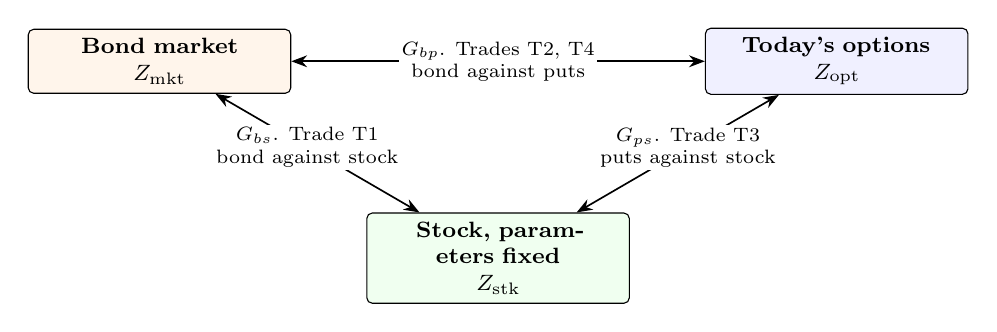
\begin{tikzpicture}[font=\footnotesize,node distance=3cm,
  v/.style={draw,rounded corners=2pt,align=center,fill=white,text width=3.1cm},
  e/.style={semithick,<->,>={Stealth[length=2mm]}},
  l/.style={font=\scriptsize,align=center,fill=white,inner sep=1pt}]
\node[v,fill=orange!8] (b) at (0,0) {\textbf{Bond market}\\ $\Zm$};
\node[v,fill=blue!6] (o) at (8.6,0) {\textbf{Today's options}\\ $\Zo$};
\node[v,fill=green!6] (s) at (4.3,-2.5) {\textbf{Stock, parameters fixed}\\ $\Zs$};
\draw[e] (b)--node[l]{$\Gbp$. Trades T2, T4\\ bond against puts} (o);
\draw[e] (b)--node[l,pos=0.45]{$\Gbs$. Trade T1\\ bond against stock} (s);
\draw[e] (o)--node[l,pos=0.45]{$\Gps$. Trade T3\\ puts against stock} (s);
\end{tikzpicture}
\caption{Three markets, two independent gaps: $\Gbs=\Gbp+\Gps$. If only one edge fires, that market pair has a disagreement the third does not share.}
\end{figure}

\begin{table}[ht]
\centering\footnotesize
\begin{tabularx}{\textwidth}{@{}>{\raggedright\arraybackslash}p{1.7cm}>{\raggedright\arraybackslash}p{1.7cm}>{\raggedright\arraybackslash}X>{\raggedright\arraybackslash}X@{}}
\toprule
$\Gbp$ & $\Gbs$ & Reading & Action\\
\midrule
$>+g$ & $>+g$ & Bond wide against both. The bond is the outlier & Long bond: T1, or T2 or T4 if puts are liquid\\
$<-g$ & $<-g$ & Bond tight against both & Short bond: T1 reversed, if the bond can be borrowed\\
$\approx0$ & $>+g$ & Bond and options agree. Fixed $\sigma_0$ is stale & No trade. Update $\sigma_0$. This is Yu's ``vol estimate too low'' case\\
$>+g$ & $\approx0$ & Options low against bond and stock & Buy vol: T3 long side, or T2\\
$<-g$ & $\approx0$ & Options high against bond and stock & Sell vol: T3 short side, with a jump limit\\
\bottomrule
\end{tabularx}
\caption{Decision table for step 30. $g$ starts at 0.405. \ADAPT}
\label{tab:decide}
\end{table}

\textbf{Evidence on direction.} The strongest is Chen, Chen and Li (2026). In 1980--2022, the top DES quintile of bonds beats the bottom, and the bottom quintile of stocks beats the top. So a wide bond against the stock means long bond, short stock, which is the direction of T1 and of Yu.
\begin{itemize}[nosep]
\item \textbf{Stocks.} Low minus high: 6.56\% a year, $t=3.79$ value-weighted and 3.51 equal-weighted (p.2007).
\item \textbf{Bonds, full sample.} High minus low: 5.28\% a year, $t=5.64$ value-weighted, and 6.58\%, $t=6.02$ equal-weighted, in Table IV (p.2026). The paper's introduction prints 5.57\% and 5.25\% for the same sort (p.2007). I use the table.
\item \textbf{Bonds, clean returns, 2002--2021.} 3.24\% a year, $t=2.69$, value-weighted (p.2020, note 9). This is the number to plan around. It is gross.
\item \textbf{What the paper does not show.} I find no return net of cost and no combined stock-and-bond portfolio in its text. I did not read its Internet Appendix.
\item \textbf{Two other reads.} Cao et al.\ (2023) find a 0.60\% monthly lag in bonds after a rise in implied vol, and they find no such effect in stocks. Kapadia and Pu (2012, p.544) find convergence trades earned about 6\% a year over 2001--2009. Carr and Wu (pp.492--494) find deviations predict both markets.
\end{itemize}
These are reasons to test, not expected results.

\textbf{P\&L, per leg, close to close.} $s=+1$ for a long bond. $n_s,n_p,n_c$ are signed. $\rho_b$ is repo for a long and repo less fee for a short. $\rho_s$ is cash less fee if $n_s<0$, and cash if $n_s>0$.
\begin{align*}
\text{Bond} &= sF\,(P_t-P_{t-1}+\text{coupon}_t) - sF\,P_{t-1}\rho_b\Delta t\\
\text{Stock} &= n_s(S_t-S_{t-1}+\text{div}_t) - n_sS_{t-1}\rho_s\Delta t\\
\text{Put} &= n_p(\text{Put}_t-\text{Put}_{t-1}) - n_p\text{Put}_{t-1}\,r_{\text{cash}}\Delta t,\quad\text{likewise Call}\\
\text{Treasury} &= -sh\,(T_t-T_{t-1}+\text{coupon}^T_t) + sh\,T_{t-1}\,\text{repo}\,\Delta t\\
\text{Costs} &= \text{half-spread on each leg, at entry, exit, every rebalance and every option roll}
\end{align*}

\needspace{6\baselineskip}
\subsection*{T0. Monthly rank book of bonds and stocks. Build first}
\textit{Source: signal and sort \ADAPT, from Chen, Chen and Li (2026). No part of this is in the deck. It uses the deck's idea of comparing the formula with the market (slide 26).}
\begin{description}[style=sameline,leftmargin=1.9cm,labelwidth=1.7cm,labelsep=0.2cm,itemsep=1pt,parsep=0pt,font=\bfseries]
\item[Legs] Long top-quintile bonds, short bottom-quintile bonds. Short top-quintile stocks, long bottom-quintile stocks. Treasury overlay on net duration.
\item[Size] Equal or lagged-value weight in each quintile. The paper reports each market as its own long-short portfolio. Running both together is my addition, so test the bond leg and the stock leg apart first.
\item[Hedge] Across names only. No name-level delta hedge in the base case. Rates by duration.
\item[Carry] Bond: coupon less repo on longs, coupon and fee on shorts. Stock: rebate less fee on shorts, financing on longs.
\item[Signal] Step 24a quintile, with \fn{sibling_confirms} and the $\Delta$ImpVOL skip as variants.
\item[Exit] Rebalance monthly. Test 1, 3 and 6 month holds, and hold-off bands to cut turnover.
\item[Goes wrong] (1) Costs: Cao et al.\ (p.1394) use bond bid-ask costs of 18 bp for \$1mm trades and 68 bp for \$100k, and their signal fails at the higher number. (2) Short bonds may not be borrowable. Without them, the bond leg is a long-only tilt with credit beta. (3) The edge concentrates in small bonds and high-fee stocks. (4) A single default or buyout is not hedged by name. (5) The stock leg may be partly a value premium (p.2035).
\end{description}

\needspace{6\baselineskip}
\subsection*{T1. Bond against stock}
\textit{Source: hedge \DECK{21}. Signal form \YU. Bond version \ADAPT. Filter \ADAPT.}
\begin{description}[style=sameline,leftmargin=1.9cm,labelwidth=1.7cm,labelsep=0.2cm,itemsep=1pt,parsep=0pt,font=\bfseries]
\item[Legs] Long bond, short stock, short Treasury. Reverse on the other side.
\item[Size] $F=A_{5y}/D_b$. $n_s=-sF\delta_P$. $h=F\cdot$\fn{rate_hedge_face}.
\item[Hedge] Stock for delta. Treasury for rates. No vega or jump hedge.
\item[Carry] Long side: coupon, less repo on $P$, plus rebate on the short, less dividends. GX before the stock: $9.50-4.24=+5.26$ a year per \$100.
\item[Signal] $\Gbs$ beyond $g$, with $\Gbp$ of the same sign. The filter rejects a stale $\sigma_0$. A name with no usable options runs on $\Gbs$ alone with the fallback vol, which is close to Yu.
\item[Exit] Gap crosses zero, 180 days, account below zero, or a forced event, by \fn{bond_exit_reason}. Your plan document adds a stop at 3 times the target, and Kim's scanned deck suggests a 5 standard deviation stop. Neither was tested, so run them as variants \OWN. Test a 3-month hold beside 180 days.
\item[Goes wrong] (1) Default: the hedge covers only part of the jump, 25\% to 93\% on the GX bond. (2) A buyout lifts the stock and hurts the bond, Yu's ``sure case of divergence''. (3) Short gamma as $S$ falls. (4) Bond costs: a typical Yu trade earned 1\% to 3\% on capital, and the planning cost is also 1\% to 3\%.
\end{description}

\needspace{6\baselineskip}
\subsection*{T2. Bond against put}
\textit{Source: structure \DECK{23}. Signal \ADAPT, on the idea of Carr and Wu and Chan et al.}
\begin{description}[style=sameline,leftmargin=1.9cm,labelwidth=1.7cm,labelsep=0.2cm,itemsep=1pt,parsep=0pt,font=\bfseries]
\item[Legs] Long bond, long puts, stock to zero the delta, short Treasury.
\item[Size] Default-loss form, slide 23: solve $\begin{pmatrix}\delta_p&1\\J_p&-S\end{pmatrix}\begin{pmatrix}n_p\\n_s\end{pmatrix}=\begin{pmatrix}-F\delta_P\\F(P-100R_b)\end{pmatrix}$, with $F$ in units of \$100 of face. Market-value form, Avino and Salvador: $n_p=F\delta_P/|\delta_p|$, with no stock.
\item[Compare] Near the barrier the two forms agree. On GX, the market-value form takes 12.04 of the 7.5 puts (\$30.3), and they cover 95\% of the jump. Further away they differ. On slide 21 it takes 2.90 puts (\$15.1) and covers 71\%. In Avino and Salvador's mostly BBB and A sample the gap is wide: 94 puts costing \$13,283 against 1,064 puts costing \$122,605 per \$10mm (p.93). So their market-value hedge is 89\% cheaper, and it leaves most of the default loss open. Their default-loss hedge, in turn, raises hedging error on market value by well over 100\% (p.76). Pick the form by the risk you want flat. For a trade that may hold to default, use slide 23. For a short convergence trade, use the market-value form.
\item[Hedge] Delta and jump are flat at entry. Vega stays open. On GX it is net short: $-62.25+13.63\times3.50=-14.5$ per 1.00 scale of vol.
\item[Carry] Usually negative. GX per \$100, $K=7.5$, 2.59y: bond $+5.26$, put theta $13.63\times(-0.506)=-6.90$, stock financing $-0.19$. Total about $-1.83$ a year, before gamma gains.
\item[Signal] $\Gbp>g$ on $\Zm$, confirmed by $\PDbond>\PDopt$ at $T^*$. Variant: combine stock and put by the change in the vol skew (Avino and Salvador, pp.5, 35).
\item[Exit] $\Gbp$ crosses zero. 30 days before put expiry, roll or close. Also T1's exits.
\item[Goes wrong] (1) Term mismatch: the put expires first, so later defaults are unhedged. (2) Costs: Chan et al.\ report mean put bid-ask of 0.09 on a mean price of 0.44 (p.196), and their simple strategy goes from $+18.3\%$ to $-8\%$ a trade after costs (pp.205--206). (3) Only about one third of pairs converge (Chan, p.189). (4) A low-delta put can lose while credit is unchanged, if vol falls. (5) The old edge may be gone: practitioners viewed sell-CDS, buy-put as profitable, and Carr and Wu find the bias disappears after mid-2007 (p.488). (6) The hedging gain is modest. Model put ratios cut error by 19\% against 14\% for stock, and empirical ratios by about 25\% for both (Avino and Salvador, p.29). In their lowest-rated group, stock does up to 10\% better.
\end{description}

\needspace{6\baselineskip}
\subsection*{T3. Put against stock, with bond as the reference}
\textit{Source: idea \DECK{2, 9}, the ``flip side''. Structure and signal \ADAPT.}
\begin{description}[style=sameline,leftmargin=1.9cm,labelwidth=1.7cm,labelsep=0.2cm,itemsep=1pt,parsep=0pt,font=\bfseries]
\item[Legs] Low-strike put against ATM put, delta-hedged with stock. No bond position.
\item[Reference] $B_{\text{credit}}$: the barrier at which step 15 reprices the bond, at today's ATM-fitted vol. It implies a model skew $\sigma^M(K;B_{\text{credit}})$ (slide 9).
\item[Size] Choose vega target $N$. $n_{\text{low}}=N/\nu_{\text{low}}$. $n_{\text{ATM}}=-n_{\text{low}}\nu_{\text{low}}/\nu_{\text{ATM}}$. $n_s=-(n_{\text{low}}\delta_{\text{low}}+n_{\text{ATM}}\delta_{\text{ATM}})$.
\item[Signal] $\sigma_{\text{mkt}}(K)-\sigma^M(K;B_{\text{credit}})$ beyond 3 vol points, in either direction. 3 is my judgement. Slide 8's model-to-market gaps run up to 2.1 vol points.
\item[Carry] Option theta net of the ATM leg, plus stock financing.
\item[Exit] Vol gap inside 1 point, 30 days before expiry, or a jump-loss limit.
\item[Goes wrong] (1) A short low-strike put loses about $Ke^{-rT}$ in default. Cap it. (2) Skew also carries demand and a vol risk premium, not only credit. Cremers et al.\ (PDF p.9) find individual skew very volatile. (3) In your 2007 screen, risk reversal passed the fit test on 229 names, fewer than stock (311) or ATM vol (308).
\end{description}

\needspace{6\baselineskip}
\subsection*{T4. All three together}
\textit{Source: structure \DECK{24, 25}. Applied to a bond and with a signal \ADAPT.}
\begin{description}[style=sameline,leftmargin=1.9cm,labelwidth=1.7cm,labelsep=0.2cm,itemsep=1pt,parsep=0pt,font=\bfseries]
\item[Legs] Long bond, long put, short stock, long call (slide 24). Or long bond, long put at $K^*$, long stock (slide 25).
\item[Size] Solve $M\,n=-g$ with rows for delta, vega and jump, and columns for put, stock and call.
\item[Hedge] Delta, vega and jump are flat at entry. The residual is the spread gap itself, gamma, recovery and term mismatch.
\item[Carry] Coupon less financing, less option theta on two legs. Usually the most negative of the four.
\item[Signal] Same as T2. Use T4 when the guards in step 27 pass.
\item[Exit] Same as T2. Rebalance option legs only if the residual vega exceeds a limit.
\item[Goes wrong] (1) The solve can fail: GX with a 7.5 put and a 15 call fails the sign check. The deck's example works at $S/B=2.67$, and GX sits at 1.75. (2) Four legs mean four costs. (3) Greeks are only flat at the starting $S$. (4) Slide 25 needs a listed strike near $K^*$.
\end{description}

\textbf{Order of work.} Build T0 first, because it has published targets and needs no options. T1 next, because the machinery exists. T2 is the deck's three-instrument idea in its simplest form, so build it third. T4 only if T2's residuals warrant it. T3 last, because it needs a clean skew. The variance swap as a vega hedge appears in JPMorgan's 2007 CEV note, in Berd and Voronov (2007) and in your 2007 screen. It is not in the deck, and I leave it out.

%-----------------------------------------------------------------------------
\section{Acceptance tests}\label{sec:tests}

\textbf{Every value below comes from \fn{check_deck_numbers.py} unless marked ``to build''.} Use $r=5\%$ and $p=0$ unless stated. The deck does not print $r$ for these slides. A value of 5\% fits slides 8, 12 and 21.

{\footnotesize
\begin{longtable}{@{}>{\raggedright\arraybackslash}p{0.75cm}>{\raggedright\arraybackslash}p{6.6cm}>{\raggedright\arraybackslash}p{4.2cm}>{\raggedright\arraybackslash}p{3.3cm}@{}}
\toprule
\textbf{ID} & \textbf{Test and inputs} & \textbf{Expected} & \textbf{Tolerance}\\
\midrule\endhead
\multicolumn{4}{r}{\emph{continues}}\\\endfoot
\bottomrule\endlastfoot
\multicolumn{4}{@{}l}{\textbf{A. Limits and identities}}\\
A1 & $Q(0)$ from Eq.\ (1), remedy off. $\lambda=0$. Then $S/B=1$ and $S/B=2$ at $\lambda=0.3$ \DECK{19}. $Q(0)=1$ only at $\lambda=0$ & 1. 0.9867. 0.999867 & 1e-4\\
A2 & $Q$ never rises with $T$ & True & exact\\
A3 & \fn{fk_survival} against \fn{e2c_bond.survival}, flat vol, no remedy & Same & 1e-12\\
A4 & Eq.\ (1) equals slide 11 averaged over $B$, no cut-off. $S=15,\Bbar=15,\sigma=.25,\lambda=.3,T=1$ & 0.934494 both. With cut-off, step 13a at zero drift, 0.936004 & 1e-5\\
A5 & Knock-out part: closed form against direct integration. $K=7.5,T=1.59,\sigma=.498,B=6$ & 0.90310541 & 1e-7\\
A6 & $B\to0$: model put against Black-Scholes. $S=10.5,K=10,T=1,\sigma=.5$ & 1.5191 & 1e-3\\
A7 & $K\to0$: $P/(K\DF)$ reaches PD. GX, 2.59y & 0.2801 & 1e-3 at $K=0.001$\\
A8 & $K\to0$ call: $Se^{-pT}$. $S=10.5,T=2,p=.02$ & 10.0883 & 1e-4\\
A9 & Slide 6 chart at $S=2$ and $S=12$ & 165.0\%, 73.3\% & 0.1 pt\\
A10 & Remedy: $Q(0)=1$, $Q$ continuous at 0.5, flat hazard below & True & 1e-12\\
A11 & Step 13a at zero drift, $T=1$, $\Bbar=15$. $S=30$, then $S=5$ & 0.990967. 0.640711 & 1e-5\\
A12 & Step 11 variant as a share of $\sigma_S$. $S/D=4,1,.5,.25$ & 0.800, 0.600, 0.467, 0.360 & 1e-3\\
\multicolumn{4}{@{}l}{\textbf{B. Options against the deck}}\\
B1 & Slide 8, ten model vols. $S=10.5,B=6$, vols 49.8\%, 46.5\% & Deck's column & 0.15 vol pts each\\
B2 & Fit market vols of slide 8, one $B$, two $\sigma$ & $B=6.01$, 0.500, 0.469, rmse 0.81 & $B\pm0.25$, $\sigma\pm0.01$\\
B3 & Forward vol, 1.59y to 2.59y & 40.7\% & 0.1 pt\\
B4 & Slide 1 from two vols only, 72\%, 77\%. $r=3\%$, then $r=5\%$ & $B=6.95$, PD .1496, par 544 bp. $B=6.80$, PD .1440, par 519 bp. Deck: PD .136, par 530 bp & $\pm0.05$ on $B$, $\pm0.001$ on PD, $\pm2$ bp\\
B5 & Slide 1 from ATM 72\% and PD .136: predicted OTM vol & 76.6\% at $r=3\%$, 76.7\% at $r=5\%$. Deck 77\% & 0.1 pt against mine, 0.5 against deck\\
B6 & Slide 7. $K/F\ge0.5$, $r=0$ & $B=10$: .99, .82, .74, .70. $B=5$: .94, .82, .77, .74. $B=1$: .85, .82, .81, .80. Chart $\pm0.05$ & 0.01 against mine\\
\multicolumn{4}{@{}l}{\textbf{C. Credit against the deck}}\\
C1 & Slide 12 par curve at ten tenors. Bootstrapped vol, $R=.3$, $\lambda=0$ & 0.93, 4.84, 7.59, 8.29, 8.54, 8.67, 8.75, 8.71, 8.52, 8.27 (\%) & 20 bp against chart readings\\
C2 & Slide 12 bond, clean, flat 42\%, $R=.3$ & 83.4, 59.9, 44.5. Deck 82, 60, 43 & 1.5 points\\
C3 & Slide 14 peak, $S=1.8$, $\sigma=42\%$, to 1/3/06 & 37.7\% at $R=.3$, 48.5\% at $R=.1$. Chart $\sim$37, $\sim$47.5 & 1.5 points\\
C4 & Slide 14--15, flat hazard fit at 10/1/01, $R=.3$ & Par 30.7\% to 38.3\%. PV $-49.6$ to $-54.5$. Chart $\sim$31\%, $\sim-53$ & Chart inside the bracket\\
C5 & Slide 19 left, printed inputs & rms 50 bp to chart. At $\sigma=42\%$: 17 bp & $\le$60 bp\\
C6 & Slide 19 right, $S/B=.8$, $\sigma=17.8\%$ & rms 29 bp to chart. Printed 22.2\%: 159 bp & $\le$35 bp\\
C7 & CreditGrades Table C.1 by \fn{e2c_bond.check_table_c1} with $\times360/365$. It keeps the mass at $T=0$, so run it with the remedy off & 156 of 156. Largest gap 0.494 bp. Without the scaling 11.59 bp & 0.5 bp\\
C8 & Five rows of C.1 by the deck's Eq.\ (1), atom kept, then remedy on & 0.48 bp, then 0.99 bp & 1 bp\\
\multicolumn{4}{@{}l}{\textbf{D. Hedges against the deck}}\\
D1 & Slide 21 stock dollars at $\lambda=0$, asset vol held. Then equity vol held & $-26.9$. $-11.1$. Deck $\sim-27.4$ & Within 5\% of the deck. Equity vol must fail\\
D2 & Slides 21--25. $r=5\%$, $p=2\%$, $\lambda=.3$ on CDS, 0 on options, CDS jump 90, deck's option prices & Par 424. $-26.3$. 32.2, 29.7. 25.9, 18.8. 17.1, $-32.5$, 14.5. $K^*=39.5$. 48.2, 43.7 & 8\% against the deck's 422, $-27.4$, 32.86, 31.85, 26.4, 20.2, 17.54, $-33.27$, 14.68, 39.2, 49.13, 46.41\\
D3 & Signs on slides 22, 23, 24, 25 & $(+,+)$, $(+,+)$, $(+,-,+)$, $(+,+)$ & exact\\
D4 & After a solve, net delta, vega, jump & 0 & 1e-8\\
D5 & Delta path table in Section~\ref{sec:equity} & Shares rise. Dollars peak at 36.6. Cover 0.168 to 0.892 & 1\%\\
D6 & Guard: GX 3-leg solve with 7.5 put, 15 call & Fails the sign check. $-12.66$ puts & Must be rejected\\
D7 & Put-only hedge. Slide 21, then GX $K=7.5$, 2.59y & 2.90 puts, \$15.1, 71\% of jump. 12.04 puts, \$30.3, 95\% of jump & 1\%\\
\multicolumn{4}{@{}l}{\textbf{E. Worked example, Appendix~\ref{app:gx}}}\\
E1 & GX 6/14/01 spreads. Identity $\Gbs=\Gbp+\Gps$ & 724, 787, 736 bp. $-0.084$, $+0.066$, $-0.017$ & 1 bp. Identity 1e-10\\
E2 & $\kappa$, $R^*$, $c$, $h_b$ & 0.908, 0.356, 0.953, 0.1077 & 0.002\\
E3 & DES form on GX. Step 13a, $D=14.2$, $\sigma_S=82.2\%$, $R=.35$. Payout .03, then .05 & $-149$ bp, ratio 0.919. $-213$ bp, ratio 0.888 & 2 bp\\
\multicolumn{4}{@{}l}{\textbf{F. Pipeline tests, to build}}\\
F1 & Quotes generated from known $B,\scum$, noise $\pm1$ vol pt, then calibrated & Recover $B$ and PD & $B\pm15\%$, PD $\pm0.02$\\
F2 & Market bond price set to model price & No signal, zero trades. \fn{check_no_signal_without_gap} & exact\\
F3 & Known gap closes, nothing else moves. \fn{check_known_gap_profit}, \fn{check_legs_add_up} & P\&L equals price change less costs, financing & 1 cent\\
F4 & Run to $t$, then $t+100$. \fn{check_no_lookahead} & Same results to $t$ & exact\\
F5 & Entry lag 0, 1, 2, 5. \fn{lag_sensitivity} & If profit vanishes at lag 1, it was bounce & report\\
F6 & Each bond on another issuer's stock and options. \fn{placebo_panel} & No signal value & report\\
F7 & American grid pricer at $r=0$, no dividends & Equals the European price & 1e-3\\
F8 & Bond delta from data. \fn{empirical_hedge_slope} & Compare with model delta & report\\
F9 & On CDS if available: Lardy's printed slides 19, 25, 26 & 50\% of relative basis within $\pm$20\%. Change correlation rises with risk. Pairwise noise correlation near 0.15 & Shape only\\
F10 & Replicate Chen, Chen and Li on your sample & Quintile gaps $-139$ to $+271$ bp. Price ratio 0.94 to 1.16. Bonds up and stocks down in the top quintile. Bond premium near 3.24\% a year after 2002 & Signs must match. Sizes as shape, if samples differ\\
F11 & Slope of credit change on put return times the model ratio & Near 1. Avino and Salvador: 1.02, $t$ against one of 0.24, on CDS (p.23) & report\\
F12 & Top minus bottom $\Delta$ImpVOL decile of bonds, next month & Negative. Cao et al.: $-0.60\%$, $|t|=3.62$ & Sign must match\\
\end{longtable}}

\subsection*{Deck numbers that do not reproduce, with the likely reason}

The reasons are my reading. The deck does not confirm any of them.

\begin{enumerate}[nosep]
\item \textbf{Puts 4.92 and 2.72.} At the printed 3\% they come out 5.24 and 2.93. Annual or continuous compounding makes no real difference. A single rate of 4.78\% gives 4.91 and 2.73. The rest of the deck fits a rate near 5\%. So the printed IR may not be the rate used. The discount in the next line does use 3\%.
\item \textbf{1.90.} The slide's own formula gives 1.92. It is 1.2\% off, so this may be rounding.
\item \textbf{1.42.} The same formula gives 1.35. Any $K\times\mathrm{PD}\times\DF$ rule makes 1.42/1.90 equal 10.5/15, and it is 0.747 against 0.700. The undiscounted 10.5 $\times$ 0.136 = 1.43 is the nearest match.
\item \textbf{13.6\% does reproduce, but only with annual premiums.} A flat hazard gives 14.05\%. Quarterly gives 13.93\%. Annual, default at period end, gives 13.58\%.
\item \textbf{Slide 7.} Low-strike levels sit below mine by 0.1 to 0.2. They match if the strike axis is read one 0.05 step lower. The partly hidden caption does not describe the chart.
\item \textbf{Slide 10.} The asset vol line stays near 75\% to 80\%. With $B=6.9$ and the charted ATM vol and stock price, I get about 54\% by day 240. A $B$ of 2 to 3 keeps asset vol flattest. So the slide's stability claim is not confirmed. It matters because slides 12--15 hold $\sigma$ fixed for 15 months.
\item \textbf{Slide 19 right.} 22.2\% is 40\%/1.8, which treats 0.8 as $B/S$. The chart itself fits $S/B=0.8$ with $\sigma=17.8\%$.
\item \textbf{Slide 21's 422 bp} needs $\lambda$ near 0.28. At $\lambda=0$ it is 408 bp. The deck does not state $\lambda$ there.
\item \textbf{Slide 12's third bond.} 46.3 full and 42.7 clean with the bootstrapped vol, against 43. No single convention hits all three dates. The slide does not say clean or full.
\end{enumerate}

%-----------------------------------------------------------------------------
\section{Build plan}\label{sec:build}

\textbf{First package: WP1.} It costs little and everything depends on it. It turns the check script into a tested library. \textbf{First empirical run: WP6a.} It needs only bonds, stocks and accounts, and it has published targets, so it should come before any option data. After it, WP2, WP3, WP4 and WP8 are independent and can run in parallel. Sizes are rough estimates of focused work.

{\footnotesize
\begin{longtable}{@{}>{\raggedright\arraybackslash}p{0.8cm}>{\raggedright\arraybackslash}p{5.0cm}>{\raggedright\arraybackslash}p{1.5cm}>{\raggedright\arraybackslash}p{1.4cm}>{\raggedright\arraybackslash}p{6.2cm}@{}}
\toprule
\textbf{WP} & \textbf{Produces} & \textbf{Needs} & \textbf{Size} & \textbf{Done when}\\
\midrule\endhead
\multicolumn{5}{r}{\emph{continues}}\\\endfoot
\bottomrule\endlastfoot
\textbf{WP1} & \fn{fk_model.py}, tests. Steps 12, 13, 13a, 16. Black-Scholes helpers & Nothing & 1--2 days & A1--A12, B1--B6 pass. No market data used\\
WP2 & \fn{fk_value.py}. Steps 14, 15, 18--21, 23, 24 & WP1, \fn{e2c_bond} & 1--2 days & C1--C8, E1--E3 pass. \fn{fk_bond_price} equals \fn{risky_bond_price} at flat vol with remedy off\\
WP3 & \fn{fk_risk.py}. Steps 26--29 & WP1, WP2 & 1--2 days & D1--D7 pass\\
WP6a & \fn{fk_des.py}. Steps 1, 2, 7, 11, 17, 24a. T0 returns. Replication on your sample, no options & WP2 & 3--5 days & F10 passes on signs. A note gives gross returns by bond size and fee, and net at measured costs. If signs fail, stop and debug before any option work\\
WP4 & \fn{fk_options.py}. Steps 3--6, on synthetic quotes first & WP1 & 2--3 days & Synthetic American quotes round-trip. Bad quotes rejected. Forward recovered within 1 bp of carry\\
WP5 & \fn{fk_calibrate.py}. Steps 7--11, 22 & WP1, WP4 & 2 days & F1 passes. $U_p$ matches the Carr-Wu formula on a hand case\\
WP6 & \fn{fk_gaps.py}. Steps 25, 24b, wired to steps 18--24 & WP5, WP6a & 2 days & Gaps run on a synthetic panel. F2 passes\\
WP7 & \fn{fk_trades.py}, \fn{fk_backtest.py}. Steps 30--34. T1, then T2 & WP3, WP6 & 3--5 days & F3--F6, F11, F12 pass for T1 and T2. Leg P\&L sums to the account every day\\
WP8 & \fn{fk_american.py}. Grid pricer on $V$ with absorbing barrier & WP1 & 2 days & F7 passes. A note states the de-American error on GX inputs, and whether the base case stands\\
WP9 & First option run on 20--50 high yield names, with reports & WP4--WP7 & 2--4 days & A table of gaps, hedge slopes (F8), $P/K$ linearity test, and asset vol stability. Slide 10's claim settled for this sample. A test of whether $\Zm-\Zo$ adds to $\Zm-\Zs$\\
WP10 & Full backtest, T3 and T4 if earned, written report & WP8, WP9 & 1--2 weeks & Net Sharpe, $t$, drawdown, break-even cost, by trade type and rating. Costs at 1, 2 and 3 times measured. Any rule grid reported with overfitting probability and deflated Sharpe\\
\end{longtable}}

\textbf{Stop rules.} Stop and report if WP6a's net bond return at measured costs is zero or negative at the large-bond end. Do the same if WP9's empirical hedge slope is far from model delta. A fixed trigger is not a good stop test, since its firing rate depends on the parameters. On GX the log gap is 0.02 to 0.08 in size on the deck's values, and 0.19 to 0.26 on the published settings.

%-----------------------------------------------------------------------------
\section{Open questions and risks}\label{sec:questions}

\subsection*{Open questions, ranked, with my recommendation}

\begin{enumerate}[itemsep=3pt]
\item \textbf{Signal: a monthly rank, or a fixed trigger per name?} This decides the whole trading layer. \textbf{Use the rank as the base, and keep the trigger as a variant.} The rank has the published result. A fixed ratio test is biased at a fixed $\Lbar$, because the typical gap is not zero: Chen, Chen and Li's middle quintile has a log ratio of 1.17. Yu avoids that by fitting $\Lbar$ to each name's first ten days, which adds a fitted number and turns the signal into a change since the fit. The gap's level also moves with parameters. On GX it is $-12$ bp on the deck's values, and $-149$ to $-213$ bp on the published ones. A rank should be less exposed to that, though I have not tested it.
\item \textbf{Barrier: from each name's skew, or $\Lbar D$?} Every number depends on it, and the deck allows both. \textbf{Use $\Lbar D$ with $\Lbar=0.5$ by default.} Chen, Chen and Li get their result with exactly that (p.2015). Use the skew fit only if it improves rmse by 0.5 vol points or more and stays in $[0.25D,D]$. On GX the fit gives 6.01 and $\Lbar D$ gives 7.1. The rmse differs by about 0.16 vol points and the 2.59-year default probability by about 0.012. So the skew adds little where it can be read, and it will be noisier where quotes are thin. On GX this rule picks $B=7.1$, not the deck's 6. Tests that reproduce the deck pass $B$ in directly. Confirm in WP9.
\item \textbf{Daily refit, or hold parameters?} The deck does both: it fits on 6/14/01 and holds through 10/1/01. \textbf{Compute both.} $\Zo$ uses the refit, $\Zs$ uses the hold. On name-by-name trades, require both to agree. On the rank book, start with the $\Zs$ form and test whether the $\Zo$ form adds to it. The literature review (gap 4) says nobody has tested implied vol change, CDS momentum and the debt-equity spread together.
\item \textbf{$\lambda$ in credit and in options?} The deck fits 0 on GX and about 0.28 on the hedge example. It prints no option formula with $\lambda$. \textbf{Use 0.3 on the credit curve with the slide 19 remedy, and 0 on options.} Slides 21--25 reproduce best this way. Run $\lambda=0$ on credit as a sensitivity. It is an inconsistent pair of assumptions, and at short tenors it matters: 468 bp against 566 bp at 2 years on slide 19's left panel.
\item \textbf{Recovery?} \textbf{Use 0.40 for senior unsecured, 0.35 in the replication, report $R^*$ daily, and run 0.10 to 0.50.} Bond-specific recovery needs a source I do not have. B\'egin et al.\ (p.123) call a fixed recovery popular but inadequate.
\item \textbf{Which names?} \textbf{High yield first, BB and below, non-financial, not captive finance.} Lardy's correlation evidence and the literature review both point there. The own files show GM and Ford have no solution with this formula.
\item \textbf{American correction?} \textbf{Start with the tree plus default-leg correction, then let WP8 decide.} The effect is 1.8\% to 4.2\% of the put on GX.
\item \textbf{What about your cross-section?} \textbf{Run it as a variant of the rank.} Your weekly regression on $\ln(S/D)$ is your strongest result, at gross Sharpe 2.51. That falls to 0.62 at 5\% round-trip costs at real turnover, with no hold-out. Chen, Chen and Li find a linear mix of model inputs does not reproduce DES (p.2031). So rank the model gap first, then test whether the regression residual adds to it.
\end{enumerate}

\subsection*{Risks}

\textbf{Where the method is likely to fail.}
\begin{enumerate}[nosep]
\item \textbf{The published result may not transfer.} DES is a stock-only signal on 1980--2022 data, gross. Its bond premium on clean data after 2002 is about 60\% of the full-sample figure. Nothing in these sources tests an option-calibrated model on bonds. Chen, Chen and Li cite one out-of-sample study (Deng, Hou and Shi, 2025), which I have not read.
\item \textbf{Thin evidence.} The deck tests two names. Both lost most of their equity value in the sample (slides 10, 13). A falling stock drives the model spread up in any structural model. So tracking on those paths does not show much about a name with a stable stock.
\item \textbf{Asset vol stability is unconfirmed.} Slide 10 does not reproduce at the end of its sample with its own $B$.
\item \textbf{Near the barrier.} Slide 18 excludes ``super-depressed'' stocks. At $S/\Bbar=0.33$, $T=1$, Eq.\ (1) gives 0.601 and step 13a gives 0.641.
\item \textbf{Term mismatch.} Option data stop early, and bonds run longer. The long end of $Q$ rests on a flat-forward assumption. On GX, flat 46.5\% against the bootstrapped curve moves the 5-year par by 74 bp.
\item \textbf{Debt.} $D$ is stale between filings, and it can hide off-balance-sheet debt (CreditGrades WorldCom case, p.35).
\item \textbf{Captive finance, financials.} No solution for GM, Ford and others \OWN. Yu excludes financials and utilities (PDF p.16).
\item \textbf{Events.} Buyouts lift the stock and hurt the bond (Yu, PDF p.12). Calls change the cash flows.
\item \textbf{Bond costs may exceed the edge.} See Part 9 of \fn{02_bond_vol_method.md}. In the rerun of your workbooks, a one-week lag cuts Sharpe from 2.51 to 1.47.
\item \textbf{Model choice.} Ju et al.\ (2015) find an extended Geske-Johnson model beats CreditGrades for this trade on 369 obligors, 2004--2008. Finkelstein's model shares CreditGrades' constant barrier.
\end{enumerate}

\textbf{The deck's date and context.} It is a client presentation from June 2002, by a firm that states it makes markets in the fixed income securities it discusses (PDF p.28). Its examples come from two names whose stocks collapsed in 2000--2001. It reports no costs. Its claim that basis risk and costs are ``manageable'' (slide 26) has no supporting number in the deck.

\textbf{Market changes after 2002 that these sources support.}
\begin{itemize}[nosep]
\item \textbf{CDS contracts changed.} The market moved toward central clearing, upfront payments and fixed coupons (Carr and Wu, p.481, note 3, and Chan et al., p.194). A market par curve now needs conversion, if CDS is used as a check.
\item \textbf{CDS shrank.} Notional peaked at USD 62 trillion at end 2007 and fell to USD 25 trillion by August 2012 (Avino and Lazar, 2020, p.75).
\item \textbf{Option markets changed.} A penny pilot began (Carr and Wu, p.483, note 4). Deep out-of-the-money puts had two to four ticks of spread before it. A listed credit event binary option launched in 2007 and failed (p.476).
\item \textbf{The classic trade decayed.} Standard capital structure arbitrage shows negative Sharpe ratios both before and during the 2007--2008 crisis (Avino and Lazar, p.83). Hedging with equity was effective only before the crisis (p.77). Yu's own Sharpes on 2001--2004 data were 0.15 to 0.89. The rank form looks better on one count: Chen, Chen and Li's bond premium stays significant after 2002, at a lower level, before costs. The samples and return definitions differ, so this is not a clean comparison.
\item \textbf{Bond liquidity.} Dealers cut back liquidity as losses and funding pressure rise, and arbitrage unwinds can widen mispricing (Choi, Shachar and Shin, 2019, abstract). Bond price errors can create false premia (Dickerson et al.\ 2026, through \fn{02_bond_vol_method.md}).
\item \textbf{Limits to arbitrage.} Discrepancies are common: 41\% of five-day moves (Kapadia and Pu, 2012, p.544). The authors link integration to liquidity and idiosyncratic risk.
\end{itemize}

%-----------------------------------------------------------------------------
\appendix
\section{Worked example on the deck's numbers: GX on 14 June 2001}\label{app:gx}

\textbf{This shows the arithmetic only. It is not evidence the trade works.} Inputs from the deck: $S=10.5$, $B=6$, $R=0.30$, bond 9.5\% of 11/15/2009 at 84, vols 49.8\% and 46.5\%, fixed $\sigma_0=42\%$. Assumed: $r=5\%$, $p=0$, $\lambda=0$, 84 is a clean price. Full price is 84.77. Regenerate with section K of the check script.

\begin{enumerate}[leftmargin=*,itemsep=2pt]
\item \textbf{Three spreads.} $\Zm=724$ bp. $\Zo=787$ bp, on the options curve (price 81.79). $\Zs=736$ bp, on fixed 42\% (price 84.16).
\item \textbf{Three gaps.} $\Gbp=-0.084$. $\Gps=+0.066$. $\Gbs=-0.017$. The identity holds. All sit far inside 0.405. \textbf{So no trade on this date.} That fits the deck's message that the model tracks this name.
\item \textbf{Same gap in other units.} $\kappa=0.908$. $R^*=0.356$. $c=0.953$, so bond-implied asset vol to 2.59y is 44.3\%, against 46.5\%.
\item \textbf{Default probability to 2.59y.} Options 0.280. Bond by $\kappa$ 0.258. Bond by flat hazard 0.244. Carr-Wu on the $K=5$ put 0.315.
\item \textbf{Bond risk per \$100 face.} Delta 2.697 shares, or \$28.32. Vega $-62.25$ per 1.00 scale of vol. Jump $-51.79$.
\item \textbf{Hedges with 2.59y puts.}
\begin{center}
\footnotesize
\begin{tabular}{@{}rrrrrrrr@{}}
\toprule
$K$ & Put & Delta & Vega & Jump & Theta/yr & Delta + jump: puts, stock \$ & Delta + vega: puts, stock \$\\
\midrule
5 & 1.485 & $-0.149$ & 2.60 & 2.908 & $-0.409$ & 17.41, $-1.2$ & 23.96, 9.1\\
7.5 & 2.515 & $-0.224$ & 3.50 & 4.073 & $-0.506$ & 13.63, 3.7 & 17.78, 13.5\\
10 & 3.735 & $-0.297$ & 4.14 & 5.049 & $-0.537$ & 12.16, 9.6 & 15.05, 18.6\\
\bottomrule
\end{tabular}
\end{center}
\item \textbf{Carry.} Bond 9.50 less financing 4.24 is $+5.26$ a year. The delta-and-jump hedge at $K=7.5$ costs 6.90 of theta and 0.19 of stock financing. So the package runs at about $-1.83$ a year, before any gamma gains. A hedged trade must earn that back from the gap closing.
\item \textbf{Three legs fail here.} Put 7.5, stock and call 15 gives $-12.66$ puts, $-\$191.6$ of stock and $+\$88.3$ of calls. The guard rejects it.
\item \textbf{Puts alone, matched on delta.} 18.15 of the 5 puts (\$26.9) cover 102\% of the jump. 12.04 of the 7.5 puts (\$30.3) cover 95\%. 9.08 of the 10 puts (\$33.9) cover 89\%. Near the barrier, a delta match is nearly a jump match.
\item \textbf{The same day on published settings.} Use step 13a with $D=14.2$, $\Lbar=0.5$, $\lambda=0.3$, recovery 0.35, and ATM 82.2\% standing in for 3-year vol. Asset vol is 48.9\%. Model Z is 873 bp at payout 0.03 and 936 bp at payout 0.05, against the deck-parameter 787 bp. So DES is $-149$ to $-213$ bp, near the paper's lowest quintile value of $-139$ bp. The model price is 0.92 to 0.89 of market, where that quintile averages 0.94. On these settings GX's bond looks rich against its stock. On the deck's settings it does not. That parameter sensitivity is why the base signal is a rank.
\end{enumerate}

\section{Sources}\label{app:sources}

\footnotesize
\begin{itemize}[nosep]
\item Finkelstein, V. (2002). \emph{Assessing default probabilities from equity markets}. Goldman, Sachs \& Co. \fn{E2C/evidence/drive/01_model_notes/Finkelstein.pdf}. Dated from PDF metadata.
\item Lardy, J-P. (2002). \emph{E2C}. JPMorgan Credit Derivatives Conference, January 16. \fn{E2C_JPM_CDconference.pdf}. Cited by printed slide. PDF page = printed + 1 through printed 27.
\item Finger, C. et al. (2002). \emph{CreditGrades Technical Document}. \fn{CGtechdoc.pdf}. Cited by printed page. PDF = printed + 6.
\item Yu, F. (2005). \emph{How Profitable Is Capital Structure Arbitrage?} \fn{E2C/ssrn-687436.pdf}. Cited by PDF page, as extracted in \fn{notes/paper_method/01_paper_extraction.md}.
\item Carr, P. and Wu, L. (2011). \emph{A Simple Robust Link Between American Puts and Credit Protection}. Review of Financial Studies 24(2). Cited by journal page.
\item Chan, K., Kolokolova, O., Lin, M. and Poon, S. (2023). \emph{Price convergence between credit default swap and put option}. Journal of Empirical Finance 72.
\item Cremers, M., Driessen, J., Maenhout, P. and Weinbaum, D. (2004 working paper). \emph{Individual Stock-Option Prices and Credit Spreads}. Cited by PDF page.
\item B\'egin, J-F., Boudreault, M. and Th\'eriault, M. (2023). \emph{Leveraging prices from credit and equity option markets for portfolio risk management}. Journal of Futures Markets.
\item Cao, J., Goyal, A., Xiao, X. and Zhan, X. (2023). \emph{Implied Volatility Changes and Corporate Bond Returns}. Management Science 69(3), 1375--1397. Read the method, cost and summary sections.
\item Kapadia, N. and Pu, X. (2012). \emph{Limited arbitrage between equity and credit markets}. Journal of Financial Economics 105.
\item Avino, D. and Lazar, E. (2020). \emph{Rethinking Capital Structure Arbitrage: A Price Discovery Perspective}. Journal of Alternative Investments, Spring.
\item Ju, H-S., Chen, R-R., Yeh, S-K. and Yang, T-H. (2015). \emph{Evaluation of conducting capital structure arbitrage using the multi-period extended Geske--Johnson model}. Review of Quantitative Finance and Accounting 44. Abstract.
\item Kim, G., Li, H. and Zhang, W. (2016). \emph{CDS-bond basis and bond return predictability}. Journal of Empirical Finance 38. Abstract.
\item Choi, J., Shachar, O. and Shin, S. (2019). \emph{Dealer Liquidity Provision and the Breakdown of the Law of One Price}. Management Science 65(9). Abstract.
\item Chen, H., Chen, Z. and Li, J. (2026). \emph{The Debt-Equity Spread}. Journal of Finance 81(4), 2005--2062. DOI 10.1111/jofi.70060. Read the published version from the CityU Scholars repository (CC BY). Internet Appendix not read.
\item Avino, D. and Salvador, E. (2024). \emph{Contingent Claims and Hedging of Credit Risk with Equity Options}. Review of Asset Pricing Studies 14(2), 310--348. DOI 10.1093/rapstu/raae005. Read the accepted manuscript of 5 January 2024 from the Liverpool repository, and cited by its pages, including its appended Internet Appendix. Published numbers may differ.
\item Own files: \fn{notes/own_models/02_implemented_method.md} and \fn{03_bond_and_vol.md}, which summarise your workbooks and \fn{Capital Structure Arb-1.doc}. I did not read the raw workbooks.
\item Paper method: \fn{notes/paper_method/02_bond_vol_method.md}, \fn{e2c_bond.py}.
\item Literature review: \fn{LLMWikiGeneration/wiki/wiki/analyses/capital-structure-arbitrage-literature-review.md}.
\end{itemize}

\textbf{Scanned files, read as page images.} OCR on these is unusable.
\begin{itemize}[nosep]
\item \emph{3 Steps of CDS Bond Basis} (15 pages, no stated author, handwritten notes on it). Residual basis from index and swap betas, a fitted model, simulated expected capture as the signal, and overfitting checks across entry and exit grids. Used for step 25 variant (5) and step 34. It also has order-flow slides, which I do not use.
\item \emph{Automated Capital Structure Arbitrage} (J.\ Kim, 15 pages). CreditGrades against CDS, ranked across 1,000 names and 100 input series, with cointegration tests and a 5 standard deviation stop. Used for T1's stop variant. Its Johansen table shows rank 2 of 2 series, which means both series are stationary, not that they are cointegrated. Treat that claim with care, on 94 observations.
\item \emph{Empirical Models of Single- and Multi-Name Debt-Equity Relationship} (Berd and Voronov, 2007, 19 pages). Mostly market-level GARCH and correlation models. Its slide 5 argues for structural models with parameters set by the market, which fits Finkelstein. No number used.
\item \emph{Credit Grades Model Description} (one slide). The same content as CreditGrades. No number used.
\end{itemize}
\textbf{Other files, no number used.} \emph{A Framework for Credit-Equity Investing} (Goulden, Allen and Einchcomb, JPMorgan, 19 November 2007; text search only) uses a CEV model, a z-score signal, and stock and variance swap hedges. It reports a 64\% success rate and an information ratio of 1.96 in its own back-test (p.3). \fn{Creditgrades_model.xlsm}: a one-name CreditGrades sheet, opened read-only with no macros. It uses ATM implied vol as its input vol.

\end{document}
